\documentclass[11pt]{article}
\usepackage[margin=1in]{geometry}
%%%%%%%%%%%%%%%%%%%%%%%%%%%%%%%%%%%%%%%%%%%%%%%%%%%%%%%%%%%%%%%%%%%%%%%%%%%%
\usepackage{amsmath,amssymb,amsfonts}
\usepackage{amsthm,latexsym,mathrsfs}
\usepackage{bm,bbm,dsfont}
\usepackage{color,graphicx}
\definecolor{violet}{rgb}{0.56,0,1}
\graphicspath{{figures/}}
\DeclareGraphicsExtensions{.png,.pdf}
\usepackage[config,labelfont={rm,rm},textfont=rm]{caption,subfig}
\usepackage[latin1]{inputenc}
\usepackage[english]{babel}
\usepackage{algorithm}
\usepackage{algpseudocode}
\usepackage{placeins}
\usepackage[colorlinks=true,linkcolor=blue,citecolor=blue,urlcolor=blue]{hyperref}

\theoremstyle{plain}
\newtheorem{theorem}{Theorem}[section]
\newtheorem{lemma}[theorem]{Lemma}
\newtheorem{proposition}[theorem]{Proposition}
\newtheorem{corollary}[theorem]{Corollary}

\theoremstyle{definition}
\newtheorem{problem}[theorem]{Problem}
\newtheorem{definition}[theorem]{Definition}
\newtheorem{example}[theorem]{Example}

\theoremstyle{remark}
\newtheorem{remark}[theorem]{Remark}

\renewcommand{\labelenumi}{\textbf{\arabic{enumi}.}}
\renewcommand{\labelenumii}{\textbf{\arabic{enumi}\alph{enumii}.}}
\everymath{\displaystyle}

% section numbers in headings followed by a period: "B. Title", "3.1. Title"
\makeatletter
\renewcommand\@seccntformat[1]{\csname the#1\endcsname.\quad}
\makeatother

\numberwithin{equation}{section}
\numberwithin{figure}{section}
\numberwithin{table}{section}


\title{Minimizing the spectral radius of a diagonally scaled positive matrix\thanks{Parts of this manuscript were edited with the assistance of an AI tool (Claude Opus 5.5, Anthropic). The authors are solely responsible for all proofs and statements.}}
\author{Zhilan \and John \and Yuliya \and Ludmil}
\date{}

\begin{document}

\maketitle

\begin{abstract}
    We investigate a minimization problem for the spectral radius of a positive matrix corresponding to the model of Glasser and Feng (2023) for the allocation of vaccines to subpopulations.
\end{abstract}

\tableofcontents

\section{Formulation of the problem}\label{sec-ngm}


We consider the following optimization problem: Find $\widehat\chi_k\in\mathbb{R}^{m\times n}$, $k=1:3$, such that
\begin{equation}\label{the-min-ij}
\begin{aligned}
&\left(\widehat\chi_1,\widehat\chi_2,\widehat\chi_3\right)
\in\operatorname*{arg\,min}\ \rho\left(\operatorname{NGM}(\chi_1,\chi_2,\chi_3)\right)
\quad\mbox{subject to}\\
&\sum_{j=1}^{n}\chi_{k,ij}\,\sigma_{k,ij}=b_{k,i},\qquad \chi_{k,ij}\ge 0,
\qquad k=1,2,3,\quad i=1:m,\quad j=1:n ,
\end{aligned}
\end{equation}
The indices $i=1:m$, $j=1:n$ and $k=1,2,3$ correspond to the locations, the age groups and the vaccine types, respectively.
The $b_{k,i}\ge 0$ are the quantities of available vaccines, the number of
doses of type $k$ in location $i$, and the $\sigma_{k,ij}>0$ are the sizes of
the groups that receive them. The model we follow is described by Glasser
and Feng~\cite{JZh}, and in this model $\sigma_{1,ij}$,
$\sigma_{2,ij}$ and $\sigma_{3,ij}$ are the numbers of susceptible, vaccinated
and partially protected individuals in the age group $j$ of location $i$ at
the end of the preceding week.

To simplify the notation somewhat, we write
\begin{equation}\label{flat-index}
\begin{aligned}
&\{1,\ldots,m\}\times\{1,\ldots,n\}\ni (i,j)\mapsto p=(i-1)n+j,\quad p=1:N, \quad\mbox{with}\quad N=mn,
\end{aligned}
\end{equation}
and we use this convention on and off in the text, and we introduce the notation
\begin{equation}\label{flat}
\begin{aligned}
&\bm\chi=(\chi_1,\chi_2,\chi_3)\in\mathbb{R}^{3N},\quad \chi_{k,p}=\chi_{k,ij},\quad
\sigma_{k,p}=\sigma_{k,ij},\qquad k=1,2,3,\quad p=1:N.\\
&\mbox{For a fixed $i\in\{1,\ldots,m\}$ we denote}\quad I_i=\left\{(i-1)n+1,\ldots,in\right\}.
\end{aligned}
\end{equation}
With this indexing,~\eqref{the-min-ij} becomes the following problem.

\begin{problem}\label{ngm-problem}
Find
\begin{equation}\label{the-min}
\widehat{\bm\chi}\in\operatorname*{arg\,min}\left\{\rho\left(\operatorname{NGM}(\bm\chi)\right)\;\mbox{subject to}\;\bm\chi\in\mathfrak{S}\right\}.
\end{equation}
The set of constraints $\mathfrak{S}$ is defined as
\begin{equation}\label{constraints}
\mathfrak{S}:=\bigcap_{k=1}^{3}\bigcap_{i=1}^{m}\left\{\bm\chi\in\mathbb{R}^{3N}\ :\
\sum_{p\in I_i}\chi_{k,p}\,\sigma_{k,p}=b_{k,i},\quad \chi_{k,p}\ge 0\ \mbox{for}\ p\in I_i\right\}.
\end{equation}
\end{problem}

It remains to define the $\operatorname{NGM}$ matrix.
Following~\cite{JZh},
\begin{equation}\label{ngm}
\operatorname{NGM}=\operatorname{diag}\left(\bm d(\bm\chi)\right)A_c,
\qquad A_c\in\mathbb{R}^{2N\times 2N},
\end{equation}
The matrix $A_c$ is independent of $\bm\chi$ and is assembled from the model parameters.
The dependence of $\operatorname{NGM}$ on $\bm\chi$ is through the vector
valued function $\bm d(\bm\chi)\in\mathbb{R}^{2N}$, given by
\begin{equation}\label{yz}
d_{2p-1}=y_p,\qquad d_{2p}=z_p,
\end{equation}
where $y_p$ and $z_p$ are derived from the equilibrium fractions of the
model. Following~\cite{JZh}, for $p=1:N$,
\begin{equation}\label{yz-def}
\begin{aligned}
&y_p=\widetilde s_p,\qquad
z_p=\left\lbrack(1-\varepsilon_1)+\pi_{2,p}\right\rbrack\pi_{1,p}\,\widetilde s_p,
\qquad\mbox{where}\\
&\widetilde s_p=\left\lbrack
1+\pi_{1,p}\left(1+\pi_{2,p}+\pi_{2,p}\pi_{3,p}\right)\right\rbrack^{-1},
\qquad\mbox{and}\\
&\pi_{1,p}=\frac{\chi_{1,p}}{\omega_v+\varepsilon_2\chi_{2,p}},\qquad
\pi_{2,p}=\frac{\varepsilon_2\chi_{2,p}}{\omega},\qquad
\pi_{3,p}=1+\frac{\varepsilon_3\chi_{3,p}}{\omega}.
\end{aligned}
\end{equation}
The specific formula for $A_c$ is found in Appendix~\ref{sec-reduction},
equation~\eqref{ac-assembled}.

\section{An equivalent reduced problem on a product of simplices}\label{sec-reduced}

We first reduce the order of the matrix $\operatorname{NGM}$ by half, and then we rescale the variables to map the admissible region $\mathfrak{S}$ to a product of simplices. Let us introduce the matrix 
\begin{equation}\label{p-def}
\mathscr{P}=\sum_{p=1}^{N}\left(\bm e_{2p-1}+\bm e_{2p}\right)\bm e_p^T
\in\mathbb{R}^{2N\times N}
\end{equation}
The product of this matrix by a vector repeats each component of the vector twice. 
Next, we note an identity for $\mathscr{P}^T\mathscr{P}$  and we also 
introduce $A_1\in\mathbb{R}^{N\times N}$:
\begin{equation}\label{p-identities}
\mathscr{P}^T\mathscr{P}=2I_N \quad\mbox{and define}\quad
A_1=\frac{1}{4}\,\mathscr{P}^TA_c\mathscr{P}\in\mathbb{R}^{N\times N},
\end{equation}
We then have the following equivalence of the spectral radii of the two matrices (see Theorem~\ref{reduction} in Appendix~\ref{sec-reduction}):
\begin{equation}\label{rho-equal}
\rho\left(\operatorname{diag}(\bm d)A_c\right)=\rho\left(A_1\operatorname{diag}(\bm g)\right).
\end{equation}
Here the components of $\bm g$ are, by~\eqref{yz-def},
\begin{equation}\label{g-def}
  \begin{aligned}
g_p&=y_p+z_p
=\left\lbrack 1+(1-\varepsilon_1)\pi_{1,p}+\pi_{1,p}\pi_{2,p}\right\rbrack\widetilde s_p\\
&=\frac{1+(1-\varepsilon_1)\pi_{1,p}+\pi_{1,p}\pi_{2,p}}
{1+\pi_{1,p}+\pi_{1,p}\pi_{2,p}+\pi_{1,p}\pi_{2,p}\pi_{3,p}}\ \in(0,1],
  \end{aligned}
\end{equation}
with $\pi_{1,p}$, $\pi_{2,p}$ and $\pi_{3,p}$ as in~\eqref{yz-def}. Each $g_p$
depends on $\chi_{1,p}$, $\chi_{2,p}$ and $\chi_{3,p}$.

\begin{remark}\label{rem:b}
The constraints~\eqref{constraints} decouple over the pairs $(k,i)$. If $b_{k,i}=0$ for a pair $(k,i)$, then, since $\sigma_{k,p}>0$ and $\chi_{k,p}\ge 0$, the constraint implies that $\chi_{k,p}=0$ for all $p\in I_i$. Therefore we need to consider only the pairs $(k,i)$ with $b_{k,i}>0$. The single dose of Section~\ref{sec-single} is the case $b_{2,i}=b_{3,i}=0$ for all $i$.
\end{remark}

For $b_{k,i}>0$ we change variables: for $i=1:m$ and $k=1,2,3$,
\begin{equation}\label{u-of-chihat}
  \begin{aligned}
& u_{k,p}=\frac{\sigma_{k,p}\chi_{k,p}}{b_{k,i}},\qquad
\chi_{k,p}=\frac{b_{k,i}u_{k,p}}{\sigma_{k,p}},\qquad
p\in I_i,
  \end{aligned}
\end{equation}
and, as for $\bm\chi$ in~\eqref{flat}, we also write $u_{k,ij}=u_{k,p}$.

The Problem~\ref{ngm-problem} is then equivalent to: Find $\widehat{\bm u}\in\mathbb{R}^{3N}$ such that
\begin{equation}\label{reduced-problem}
  \begin{aligned}
& \widehat{\bm u}\in\operatorname*{arg\,min}\left\{\rho\left(A_1\operatorname{diag}\left(\bm g(\bm u)\right)\right)\;\mbox{subject to}\;\bm u\in\mathcal{S}\right\},\quad\mbox{where}\\
&\mathcal{S}:=\left\{\bm u\in\mathbb{R}^{3N}\ :\ \sum_{p\in I_i}u_{k,p}=1,\quad u_{k,p}\ge 0\right\},
  \end{aligned}
\end{equation}
with $\bm g$ given by~\eqref{g-def}. We would like to point out that $\mathcal{S}$ as well as $\mathfrak{S}$ are {\bf compact and convex}. 

Furthermore, by~\eqref{ngm} and Theorem~\ref{reduction} the objective function of
Problem~\ref{ngm-problem} equals $\rho\left(A_1\operatorname{diag}(\bm g)\right)$
for every $\bm\chi\ge 0$, and $\bm\chi\in\mathfrak{S}$ if and only if
$\bm u\in\mathcal{S}$. The minimum is attained, since $\mathcal{S}$ is compact
and the objective function is continuous.

\section{Optimization for a single dose}\label{sec-single}

In this section the second and third doses are fixed,
$\bm\chi_2=\bm\theta\ge 0$ and $\bm\chi_3=\bm\zeta\ge 0$, and we minimize
$\Psi(\bm\chi_1,\bm\theta,\bm\zeta)=\rho\left(\operatorname{NGM}(\bm\chi_1,\bm\theta,\bm\zeta)\right)$ over
$\bm\chi_1$. The single dose problem, in which only doses of the first type
are available, $b_{2i}=b_{3i}=0$ for all $i$, is the case
$\bm\theta=\bm\zeta=0$, since the coefficients $\sigma_{2,p}$ and
$\sigma_{3,p}$ are positive. Throughout this section
$0<\varepsilon_l\le 1$, $l=1,2,3$. Let
\begin{equation}\label{t-coeffs}
\omega_p=\omega_v+\varepsilon_2\theta_p,\qquad
\gamma_p=1+\frac{2\varepsilon_2}{\omega}\theta_p+\frac{\varepsilon_2\varepsilon_3}{\omega^2}\theta_p\zeta_p,\qquad
e_p=\frac{1}{\gamma_p}\left(\varepsilon_1+\frac{\varepsilon_2}{\omega}\theta_p+\frac{\varepsilon_2\varepsilon_3}{\omega^2}\theta_p\zeta_p\right).
\end{equation}
Multiplying the numerator and the denominator of~\eqref{g-def} by $\omega_p>0$
and using~\eqref{yz-def} gives
\begin{equation}\label{t-PQ}
g_p=\frac{\omega_p+\left(1-\varepsilon_1+\varepsilon_2\theta_p/\omega\right)\chi_{1,p}}{\omega_p+\gamma_p\chi_{1,p}},
\end{equation}
and $1-\varepsilon_1+\varepsilon_2\theta_p/\omega=\gamma_p(1-e_p)$. Hence, with
$t_p$ as below, the denominator is $\omega_pt_p$, the numerator is
$\omega_p\left(e_p+(1-e_p)t_p\right)$, and the change of variables
\begin{equation}\label{t-def}
\begin{aligned}
&t_p=1+\frac{\gamma_p}{\omega_p}\chi_{1,p}\ \ge 1,\qquad
\chi_{1,p}=\frac{\omega_p}{\gamma_p}\left(t_p-1\right),\\
&g_p=(1-e_p)+\frac{e_p}{t_p},\qquad
A_1\operatorname{diag}(\bm g)=A_1\operatorname{diag}(\mathbbm{1}-\bm e)+A_1\operatorname{diag}(\bm e)\operatorname{diag}(\bm t)^{-1}.
\end{aligned}
\end{equation}
Here $0<e_p\le 1$, since
$\gamma_p(1-e_p)=1-\varepsilon_1+\varepsilon_2\theta_p/\omega\ge 0$; for
$\bm\theta=\bm\zeta=0$, $t_p=1+\chi_{1,p}/\omega_v$ and $e_p=\varepsilon_1$.
Then $g_p>0$ for $t_p>0$, and $g_p$ is strictly decreasing in $t_p$.
Using~\eqref{t-def} we can rewrite the problem as:
\begin{subequations}\label{t-program}
\begin{align}
&\widehat{\bm t}\in\operatorname*{arg\,min}\ \Psi(\bm t),\qquad
\Psi(\bm t)=\rho\left(A_1\operatorname{diag}(\bm g)\right),\\
&\mbox{subject to}\qquad
\sum_{p\in I_i}\widetilde\sigma_p\,t_p\le c_i,\qquad \bm t\ge\mathbbm{1},\label{t-constraint}\\
&\mbox{where}\quad \widetilde\sigma_p=\frac{\omega_p}{\omega_v\gamma_p}\sigma_{1,p},\quad
c_i=\frac{b_{1i}}{\omega_v}+\sum_{p\in I_i}\widetilde\sigma_p,
\quad\mbox{and}\quad g_p=(1-e_p)+\frac{e_p}{t_p},\quad p\in I_i,\quad i=1:m.\nonumber
\end{align}
\end{subequations}
We assume $b_{1i}>0$ for $i=1:m$: if $b_{1i}=0$ for some $i$ then,
by~\eqref{t-constraint} and $\widetilde\sigma_p>0$, we have that $t_p=1$ for all
$p\in I_i$ so these unknowns can be eliminated. We denote the set of vectors satisfying
the constraints in~\eqref{t-constraint} by $\mathcal{K}$, namely,
\begin{equation}\label{Kt-def}
\mathcal{K}=\left\{\bm t\in\mathbb{R}^N\ :\ \bm t\ \mbox{satisfies~\eqref{t-constraint}}\right\}.
\end{equation}
Notice that in the problem defined in~\eqref{t-program} the equalities
of~\eqref{constraints} have been replaced by inequalities. As we shall see in
Corollary~\ref{all-active} there is a solution to~\eqref{t-program} (a
minimizer) which satisfies all constraints
with equalities, i.e.\ all constraints are {\bf active}.

\begin{theorem}\label{active}
Let $A_1\ge 0$ with $\rho(A_1)>0$, let $\bm t\in\mathcal{K}$, and suppose that the
constraint of location $i$ in~\eqref{t-constraint} is inactive at $\bm t$,
that is, $\sum_{p\in I_i}\widetilde\sigma_pt_p<c_i$. Then:
\begin{enumerate}
\renewcommand{\labelenumi}{(\roman{enumi})}
\item there is $\widetilde{\bm t}\in\mathcal{K}$ which differs from $\bm t$ in
one component only, at which the constraint of location $i$ is active, the
other constraints of~\eqref{t-constraint} being as at $\bm t$, and
$\Psi\left(\widetilde{\bm t}\right)\le\Psi(\bm t)$;
\item if $A_1$ is irreducible, then $\Psi\left(\widetilde{\bm t}\right)<\Psi(\bm t)$,
and $\bm t$ is not a local minimizer of $\Psi$ on $\mathcal{K}$.
\end{enumerate}
\end{theorem}
\begin{proof}
Fix $q\in I_i$ and put
$\delta_{\max}=\left(c_i-\sum_{p\in I_i}\widetilde\sigma_pt_p\right)/\widetilde\sigma_q>0$.
For $0<\delta\le\delta_{\max}$ let $\bm t_\delta=\bm t+\delta\bm e_q$. Then
$\bm t_\delta\ge\bm t\ge\mathbbm{1}$, the sums of the locations other than $i$
are unchanged, and
$\sum_{p\in I_i}\widetilde\sigma_p\left(\bm t_\delta\right)_p=\sum_{p\in I_i}\widetilde\sigma_pt_p+\widetilde\sigma_q\delta\le c_i$,
with equality for $\delta=\delta_{\max}$. Hence $\bm t_\delta\in\mathcal{K}$.
Since $e_q>0$, the function $g_q=(1-e_q)+e_q/t_q$
is strictly decreasing in $t_q$, while $g_p$ for $p\neq q$ does not change.
Therefore the vector $\bm g_\delta$ at $\bm t_\delta$ satisfies
$0<\bm g_\delta\le\bm g$ and $\bm g_\delta\neq\bm g$. Hence
$0\le A_1\operatorname{diag}\left(\bm g_\delta\right)\le A_1\operatorname{diag}(\bm g)$,
and by Theorem~\ref{mono} in Appendix~\ref{sec-facts},
$\rho\left(A_1\operatorname{diag}\left(\bm g_\delta\right)\right)\le\rho\left(A_1\operatorname{diag}(\bm g)\right)$,
that is, $\Psi\left(\bm t_\delta\right)\le\Psi(\bm t)$. Taking
$\widetilde{\bm t}=\bm t_{\delta_{\max}}$ proves (i).

If $A_1$ is irreducible, then so is $A_1\operatorname{diag}(\bm g)$, and it has
no zero column, so $A_1\operatorname{diag}\left(\bm g_\delta\right)\neq A_1\operatorname{diag}(\bm g)$
and the inequality of Theorem~\ref{mono} is strict. Hence
$\Psi\left(\bm t_\delta\right)<\Psi(\bm t)$ for every $0<\delta\le\delta_{\max}$.
For $\delta=\delta_{\max}$ this is the first claim of (ii), and since
$\bm t_\delta\to\bm t$ as $\delta\to 0$, every neighbourhood of $\bm t$ contains
points of $\mathcal{K}$ with a smaller value of $\Psi$, so $\bm t$ is not a
local minimizer.
\end{proof}

\begin{corollary}\label{all-active}
Let $A_1\ge 0$ with $\rho(A_1)>0$. The minimum of $\Psi$ on $\mathcal{K}$ equals its minimum on
$\left\{\bm t\in\mathcal{K}:\sum_{p\in I_i}\widetilde\sigma_pt_p=c_i,\ i=1:m\right\}$.
In particular, $\Psi$ has a minimizer on $\mathcal{K}$ at which all $m$
constraints are active, and if $A_1$ is irreducible, then every local minimizer of $\Psi$ on
$\mathcal{K}$ meets all $m$ constraints with equality.
\end{corollary}
\begin{proof}
Start from any $\bm t\in\mathcal{K}$ and apply Theorem~\ref{active}(i) to
the inactive constraints one location at a time. A step at location $i$
changes only a component $t_q$ with $q\in I_i$, so the constraints made active
before stay active, and after at most $m$ steps we reach a point of
$\mathcal{K}$ at which all $m$ constraints are active and the value of $\Psi$
is at most $\Psi(\bm t)$. Hence the two minima are equal. The set of points of
$\mathcal{K}$ at which all $m$ constraints are active is closed and bounded,
since $1\le t_p\le c_i/\widetilde\sigma_p$ for $p\in I_i$. On it $\Psi$ is
continuous: $\bm g$ is continuous in $\bm t>0$, the spectral radius is a
continuous function of the entries, and with $\gamma=\min_p g_p>0$,
Theorem~\ref{mono} in~\S\ref{sec-facts} gives
$\rho\left(A_1\operatorname{diag}(\bm g)\right)\ge\gamma\rho(A_1)>0$. So $\Psi$
attains its minimum on this set, and by the equality of the two minima this is a
minimizer of $\Psi$ on $\mathcal{K}$. The statement on local minimizers is
Theorem~\ref{active}(ii).
\end{proof}

\begin{theorem}\label{global}
Let $A_1\ge 0$ with $\rho(A_1)>0$. Then $\Psi$ is convex and continuous
on $\mathcal{K}$, the minimum in~\eqref{t-program} is attained, and every local
minimizer is a global minimizer. If in addition $A_1$ is irreducible, then the
minimizer is unique.
% , $\Psi$ is continuously differentiable on
% $\left\{\bm t>0\right\}$, and the Karush--Kuhn--Tucker conditions are necessary
% and sufficient for a global minimum.
\end{theorem}
\begin{proof}
The feasible set $\mathcal{K}$ is closed, and bounded because $\bm t\ge\mathbbm{1}$ and
$\widetilde\sigma_p>0$ give $1\le t_p\le c_i/\widetilde\sigma_p$; it is convex, being an
intersection of half-spaces. For $\bm t>0$ one has $g_p\ge\gamma=\min_p g_p>0$, so
$A_1\operatorname{diag}(\bm g)\ge\gamma A_1$ and, by Theorem~\ref{mono}
in~\S\ref{sec-facts}, $\rho\left(A_1\operatorname{diag}(\bm g)\right)\ge\gamma\rho(A_1)>0$.
The spectral radius is a continuous function of the entries, so $\Psi$ is
continuous on $\{\bm t>0\}$.

For convexity let $\bm t\neq\bm t'$ be positive, let $0<\lambda<1$, and set
$\bm t_\lambda=\lambda\bm t+(1-\lambda)\bm t'$. We write $\bm g$, $\bm g'$ and
$\bm g_\lambda$ for the vectors $\bm g$ of~\eqref{t-def} at $\bm t$, $\bm t'$
and $\bm t_\lambda$, and $\bm g^{\lambda}\bm g'^{\,1-\lambda}$ for the vector
with components $g_p^{\lambda}g_p'^{\,1-\lambda}$. We first show
\begin{equation}\label{g-strict}
\bm g_\lambda\le\bm g^{\lambda}\bm g'^{\,1-\lambda},
\end{equation}
with strict inequality in every component $p$ for which $t_p\neq t'_p$.
Fix $p$, and write $t=t_p$, $t'=t'_p$, $a=1-e_p\ge 0$ and
$b=e_p>0$. The weighted inequality between the arithmetic and the
geometric mean gives $\lambda t+(1-\lambda)t'\ge t^{\lambda}t'^{\,1-\lambda}$,
with equality only if $t=t'$, and H\"older's inequality with exponents
$1/\lambda$ and $1/(1-\lambda)$ gives
$x_1^{\lambda}y_1^{1-\lambda}+x_2^{\lambda}y_2^{1-\lambda}\le\left(x_1+x_2\right)^{\lambda}\left(y_1+y_2\right)^{1-\lambda}$
for $x_l,y_l\ge 0$. Applying these two in turn,
\begin{equation}
\begin{aligned}
\left(\bm g_\lambda\right)_p
&=a+\frac{b}{\lambda t+(1-\lambda)t'}
\le a^{\lambda}a^{1-\lambda}+\left(\frac{b}{t}\right)^{\lambda}\left(\frac{b}{t'}\right)^{1-\lambda}\\
&\le\left(a+\frac{b}{t}\right)^{\lambda}\left(a+\frac{b}{t'}\right)^{1-\lambda}
=g_p^{\lambda}g_p'^{\,1-\lambda},
\end{aligned}
\end{equation}
and the first inequality is strict if $t\neq t'$. This
proves~\eqref{g-strict}. Lemma~\ref{log-convex} in~\S\ref{sec-facts}, applied to
the points $\bm\xi$ and $\bm\eta$ with $e^{\bm\xi}=\bm g$ and $e^{\bm\eta}=\bm g'$, states
\begin{equation}
\rho\left(A_1\operatorname{diag}\left(\bm g^{\lambda}\bm g'^{\,1-\lambda}\right)\right)
\le\rho\left(A_1\operatorname{diag}(\bm g)\right)^{\lambda}
\rho\left(A_1\operatorname{diag}(\bm g')\right)^{1-\lambda}.
\end{equation}
Therefore
\begin{equation}\label{psi-strict}
\rho\left(A_1\operatorname{diag}\left(\bm g_\lambda\right)\right)
\le\rho\left(A_1\operatorname{diag}\left(\bm g^{\lambda}\bm g'^{\,1-\lambda}\right)\right)
\le\rho\left(A_1\operatorname{diag}(\bm g)\right)^{\lambda}
\rho\left(A_1\operatorname{diag}(\bm g')\right)^{1-\lambda},
\end{equation}
where the first inequality follows from Theorem~\ref{mono}, since
by~\eqref{g-strict}
$0\le A_1\operatorname{diag}\left(\bm g_\lambda\right)\le A_1\operatorname{diag}\left(\bm g^{\lambda}\bm g'^{\,1-\lambda}\right)$.
By the weighted inequality between the arithmetic and the geometric mean, the
right-hand side of~\eqref{psi-strict} is at most
$\lambda\Psi(\bm t)+(1-\lambda)\Psi(\bm t')$, so
$\Psi\left(\bm t_\lambda\right)\le\lambda\Psi(\bm t)+(1-\lambda)\Psi(\bm t')$,
and $\Psi$ is convex. The feasible set is compact and
$\Psi$ is continuous, so the minimum is attained, and every local minimizer of
a convex function on a convex set is a global minimizer.

Let now $A_1$ be irreducible.
% For $\bm t>0$ the matrix
% $A_1\operatorname{diag}(\bm g)\ge 0$ has the same zero entries as $A_1$ and is
% irreducible, so by Theorem~\ref{pf} in~\S\ref{sec-facts} its spectral radius
% is a simple eigenvalue, hence a continuously differentiable function of the
% entries, which are continuously differentiable in $\bm t$.
The two sides of~\eqref{g-strict} being distinct, the two matrices compared
in the first inequality of~\eqref{psi-strict} are distinct, the larger one is
irreducible, and by Theorem~\ref{mono} this inequality is strict: $\Psi$ is strictly convex. If $\bm t\neq\bm t'$ were two minimizers, then
$\bm t_{1/2}$ would be feasible, the feasible set being convex, and
$\Psi\left(\bm t_{1/2}\right)$ would be smaller than the minimum; hence the
minimizer is unique.
% The Karush--Kuhn--Tucker conditions are necessary and
% sufficient for a continuously differentiable convex function on a set defined
% by affine constraints.
\end{proof}

\subsection{Optimality conditions}\label{sec-algorithm}

As is well known, a point of $\mathcal{K}$ is the minimizer if and only if it
satisfies the Karush--Kuhn--Tucker conditions; for our problem this is
Proposition~\ref{kkt-sufficient} below. Any method that computes such a point
can be used, and the conditions are checked at the computed point. A gradient method needs the gradient of
$\Psi$, and for this the eigenvectors corresponding to the spectral
radii of $A_1\operatorname{diag}(\bm g)$ and
$\left[A_1\operatorname{diag}(\bm g)\right]^T$ suffice. Let
\begin{equation}\label{perron}
A_1\operatorname{diag}(\bm g)\,\bm v=\rho\,\bm v,\qquad
\operatorname{diag}(\bm g)A_1^T\bm w=\rho\,\bm w,\qquad \bm v>0,\ \bm w>0 .
\end{equation}
Then
$\partial\rho/\partial g_p=\left(A_1^T\bm w\right)_pv_p/\langle\bm w,\bm v\rangle$,
and since $dg_p/dt_p=-e_p/t_p^2$ the chain rule gives
\begin{equation}\label{grad}
\frac{\partial\Psi}{\partial t_p}
=-\frac{e_p}{t_p^2}\cdot
\frac{\left(A_1^T\bm w\right)_p v_p}{\langle\bm w,\bm v\rangle}\ <0 ,
\end{equation}
the sign because $\bm v>0$, $\bm w>0$ and no column of $A_1$ vanishes.

With multipliers $\mu_i$ for the constraints $\sum_{p\in I_i}\widetilde\sigma_pt_p\le c_i$
and $\nu_p$ for $t_p\ge 1$, the Lagrangian is
\begin{equation}\label{lagrangian}
\mathcal{L}(\bm t,\bm\mu,\bm\nu):=\Psi(\bm t)
+\sum_{i=1}^m\mu_i\left(\sum_{p\in I_i}\widetilde\sigma_pt_p-c_i\right)
+\sum_{p=1}^N\nu_p\left(1-t_p\right).
\end{equation}
The KKT conditions for the Lagrangian are equivalent to (for $i=1:m$ and $p\in I_i$):
\begin{equation}\label{kkt}
\begin{aligned}
&\sum_{p\in I_i}\widetilde\sigma_pt_p=c_i,\qquad t_p\ge 1,\qquad \nu_p\ge 0,\qquad \nu_p\left(t_p-1\right)=0,\\
&\mu_i=\frac{1}{\widetilde\sigma_p}\left(\nu_p+\frac{e_p}{t_p^2}\cdot
\frac{\left(A_1^T\bm w\right)_pv_p}{\langle\bm w,\bm v\rangle}\right).
\end{aligned}
\end{equation}
The budget constraints are written with equality in~\eqref{kkt}, since
by Corollary~\ref{all-active} they are active at the minimizer. The fraction
in the last line of~\eqref{kkt} is positive and $\nu_p\ge 0$, so $\mu_i>0$ for
every $i$. For a coordinate with $t_p>1$ one has $\nu_p=0$, so
\begin{equation}\label{ratio}
r_p:=\frac{e_p}{t_p^2\,\widetilde\sigma_p}\cdot
\frac{\left(A_1^T\bm w\right)_pv_p}{\langle\bm w,\bm v\rangle}
\end{equation}
equals $\mu_i$ and is the same for every such $p$ at the index $i$; for a
coordinate at $t_p=1$ the ratio $r_p$ is at most $\mu_i$. That these conditions characterize the minimizer is the content
of the next proposition.

\begin{proposition}\label{kkt-sufficient}
Let $A_1\ge 0$ be irreducible. A point $\bm t\in\mathcal{K}$ is the minimizer
$\widehat{\bm t}$ of~\eqref{t-program} if and only if there are multipliers
$\mu_i$, $i=1:m$, and $\nu_p$, $p=1:N$, such that~\eqref{kkt}
holds.
\end{proposition}
\begin{proof}
For $\bm t>0$ the matrix $A_1\operatorname{diag}(\bm g)\ge 0$ has the same
zero entries as $A_1$ and is irreducible, so by Theorem~\ref{pf}
in~\S\ref{sec-facts} its spectral radius is a simple eigenvalue with the
positive eigenvectors $\bm v$ and $\bm w$ of~\eqref{perron}. A simple
eigenvalue is a differentiable function of the entries of the matrix, with
the derivative $\partial\rho/\partial g_p$ given before~\eqref{grad}; see
Horn and Johnson~\cite[Section 6.3]{1985Horn_Johnson}. The entries are differentiable in $\bm t$,
so $\Psi$ is differentiable at $\bm t$, its partial derivatives are given
by~\eqref{grad}, and~\eqref{kkt} reads
$\partial\Psi/\partial t_p(\bm t)=-\mu_i\widetilde\sigma_p+\nu_p$ for $p\in I_i$.

Let $\bm y\in\mathcal{K}$ and $0<s<1$. Since $\Psi$ is convex
(Theorem~\ref{global}),
$\Psi\left(\bm t+s(\bm y-\bm t)\right)-\Psi(\bm t)\le s\left(\Psi(\bm y)-\Psi(\bm t)\right)$.
We divide by $s$ and let $s\to 0$:
\begin{equation}
\Psi(\bm y)-\Psi(\bm t)\ge\sum_p\frac{\partial\Psi}{\partial t_p}(\bm t)\left(y_p-t_p\right)
=\sum_i\mu_i\sum_{p\in I_i}\widetilde\sigma_p\left(t_p-y_p\right)
+\sum_p\nu_p\left(y_p-t_p\right).
\end{equation}
By the KKT conditions given in~\eqref{kkt},
\begin{align*}
&\mu_i\sum_{p\in I_i}\widetilde\sigma_p\left(t_p-y_p\right)
=\mu_i\left(c_i-\sum_{p\in I_i}\widetilde\sigma_py_p\right)\ge 0,\\
&\nu_p\left(y_p-t_p\right)=\nu_p\left(y_p-1\right)\ge 0,
\end{align*}
because $\bm y\in\mathcal{K}$. Hence $\Psi(\bm y)\ge\Psi(\bm t)$ for every
$\bm y\in\mathcal{K}$, and $\bm t=\widehat{\bm t}$ by the uniqueness in
Theorem~\ref{global}.

Conversely, $\Psi$ is convex and differentiable on the open set
$\{\bm t>0\}$, which contains $\mathcal{K}$, and the constraints
of~\eqref{t-constraint} are affine and satisfied by some point, so
the Karush--Kuhn--Tucker conditions hold at the minimizer
$\widehat{\bm t}$; see Boyd and
Vandenberghe~\cite[Sections 5.2.3 and 5.5.3]{2004Boyd_Vandenberghe}. By
Corollary~\ref{all-active} the budget constraints hold with equality at
$\widehat{\bm t}$, which gives the equality in~\eqref{kkt}.
\end{proof}

\subsection{A fixed point iteration}\label{sec-fixed-point}

The conditions~\eqref{kkt} depend on $\bm t$ in two ways: explicitly, through
$t_p$, and through the eigenvectors $\bm v$ and $\bm w$ of~\eqref{perron}.
With the eigenvectors fixed, the conditions decouple over the locations and
are solved in closed form up to one scalar equation per location. For
$\bm v>0$ and $\bm w>0$ let
\begin{equation}\label{a-p}
a_p=\frac{\left(A_1^T\bm w\right)_pv_p}{\langle\bm w,\bm v\rangle}>0,
\qquad p=1:N ;
\end{equation}
$a_p$ does not change when $\bm v$ or $\bm w$ is multiplied by a positive
number.

\begin{lemma}\label{frozen}
Let $a_p>0$, $\widetilde\sigma_p>0$ for $p\in I_i$, and
$c_i>\sum_{p\in I_i}\widetilde\sigma_p$. For $\mu>0$ let
\begin{equation}\label{t-of-mu}
t_p(\mu)=\max\left\{1,\ \sqrt{\frac{e_pa_p}{\mu\,\widetilde\sigma_p}}\right\},
\qquad
F_i(\mu)=\sum_{p\in I_i}\widetilde\sigma_p\,t_p(\mu).
\end{equation}
Then the equation $F_i(\mu)=c_i$ has exactly one solution $\mu_i>0$, and the
only solution of~\eqref{kkt-frozen} below is this $\mu_i$ together with
$t_p=t_p(\mu_i)$ and
$\nu_p=\max\left\{0,\ \mu_i\widetilde\sigma_p-e_pa_p\right\}$ for $p\in I_i$:
\begin{equation}\label{kkt-frozen}
\begin{aligned}
&\sum_{p\in I_i}\widetilde\sigma_pt_p=c_i,\qquad t_p\ge 1,\qquad \nu_p\ge 0,\qquad
\nu_p\left(t_p-1\right)=0,\\
&\mu_i=\frac{1}{\widetilde\sigma_p}\left(\nu_p+\frac{e_pa_p}{t_p^2}\right),
\qquad p\in I_i .
\end{aligned}
\end{equation}
\end{lemma}
\begin{proof}
Each $t_p(\mu)$ is continuous and non-increasing in $\mu$, and strictly
decreasing where it exceeds $1$. Hence $F_i$ is continuous and
non-increasing on $(0,\infty)$, and strictly decreasing on the set where
$F_i(\mu)>\sum_{p\in I_i}\widetilde\sigma_p$, since there at least one $t_p(\mu)>1$.
As $\mu\to 0^+$, $F_i(\mu)\ge\widetilde\sigma_p\sqrt{e_pa_p/(\mu\widetilde\sigma_p)}\to\infty$
for any $p\in I_i$, and $F_i(\mu)=\sum_{p\in I_i}\widetilde\sigma_p<c_i$ for
$\mu\ge\max_{p\in I_i}e_pa_p/\widetilde\sigma_p$. By the intermediate value
theorem $F_i(\mu)=c_i$ has a solution $\mu_i>0$; it lies in the set where $F_i$ is
strictly decreasing, so it is unique.

Let $\left(t_p\right)_{p\in I_i}$, $\left(\nu_p\right)_{p\in I_i}$, $\mu_i$
solve~\eqref{kkt-frozen}. The last equation gives
$\mu_i\ge e_pa_p/(t_p^2\widetilde\sigma_p)>0$. If $t_p>1$, then $\nu_p=0$,
so $t_p^2=e_pa_p/(\mu_i\widetilde\sigma_p)$, $t_p=t_p(\mu_i)$, and
$\mu_i\widetilde\sigma_p-e_pa_p=\mu_i\widetilde\sigma_p\left(1-t_p^2\right)<0$,
so $\nu_p=0=\max\left\{0,\mu_i\widetilde\sigma_p-e_pa_p\right\}$. If $t_p=1$, then
$\nu_p=\mu_i\widetilde\sigma_p-e_pa_p\ge 0$, so
$e_pa_p/(\mu_i\widetilde\sigma_p)\le 1$, $t_p=1=t_p(\mu_i)$ and
$\nu_p=\max\left\{0,\mu_i\widetilde\sigma_p-e_pa_p\right\}$. The first
equation is then $F_i(\mu_i)=c_i$, and $\mu_i$ is its unique solution.

Conversely, for this $\mu_i$ the numbers $t_p=t_p(\mu_i)\ge 1$ and
$\nu_p=\max\left\{0,\mu_i\widetilde\sigma_p-e_pa_p\right\}\ge 0$ satisfy
the first equation of~\eqref{kkt-frozen} because $F_i(\mu_i)=c_i$. If
$e_pa_p>\mu_i\widetilde\sigma_p$, then $t_p^2=e_pa_p/(\mu_i\widetilde\sigma_p)$
and $\nu_p=0$; otherwise $t_p=1$ and $\nu_p=\mu_i\widetilde\sigma_p-e_pa_p$.
In both cases $\nu_p\left(t_p-1\right)=0$ and
$\nu_p+e_pa_p/t_p^2=\mu_i\widetilde\sigma_p$.
\end{proof}

The equation $F_i(\mu)=c_i$ is solved exactly. Let
$\beta_p=e_pa_p/\widetilde\sigma_p$ for $p\in I_i$, ordered as
$\beta_{(1)}\le\dots\le\beta_{(q)}$, $q=|I_i|$, with the same ordering of
$e_p$, $a_p$ and $\widetilde\sigma_p$, and let $\beta_{(0)}=0$. Since $t_p(\mu)=1$ for
$\mu\ge\beta_p$ and $t_p(\mu)=\sqrt{\beta_p/\mu}$ for $\mu<\beta_p$, on each
interval $\left[\beta_{(j)},\beta_{(j+1)}\right]$, $j=0:q-1$,
\begin{equation}\label{F-piece}
F_i(\mu)=C_j+\frac{B_j}{\sqrt\mu},\qquad
C_j=\sum_{l=1}^{j}\widetilde\sigma_{(l)},\qquad
B_j=\sum_{l=j+1}^{q}\sqrt{e_{(l)}a_{(l)}\widetilde\sigma_{(l)}} .
\end{equation}
Let $j$ be the largest index in $0:q-1$ with $F_i\left(\beta_{(j)}\right)\ge c_i$,
where $F_i\left(\beta_{(0)}\right)=+\infty$. Since
$F_i\left(\beta_{(q)}\right)=\sum_{p\in I_i}\widetilde\sigma_p<c_i$, one has
$F_i\left(\beta_{(j+1)}\right)<c_i$, and since $F_i$ is non-increasing and
continuous, the solution $\mu_i$ of Lemma~\ref{frozen} lies in
$\left[\beta_{(j)},\beta_{(j+1)}\right)$. There $c_i-C_j=B_j/\sqrt{\mu_i}>0$
by~\eqref{F-piece}, so
\begin{equation}\label{mu-exact}
\mu_i=\left(\frac{B_j}{c_i-C_j}\right)^2 .
\end{equation}
The cost is that of sorting $q$ numbers.

In the problem~\eqref{t-program} one has $\widetilde\sigma_p>0$ and
$c_i-\sum_{p\in I_i}\widetilde\sigma_p=b_{1i}/\omega_v>0$, so
Lemma~\ref{frozen} applies to every location. This gives
Algorithm~\ref{alg-fixed-point}.

\begin{algorithm}[ht]
\caption{Fixed point iteration for~\eqref{kkt}}\label{alg-fixed-point}
\begin{algorithmic}[1]
\Require a start $\bm t^{(0)}\in\mathcal{K}$; a tolerance $\mathrm{tol}$ and a
maximal number of iterations $n_{iter}$
\For{$k=0,1,\ldots,n_{iter}-1$}
  \State $\bm g\gets\bm g\left(\bm t^{(k)}\right)$
  \State compute $\bm v>0$ and $\bm w>0$ such that
  $A_1\operatorname{diag}(\bm g)\,\bm v=\rho^{(k)}\bm v$ and
  $\operatorname{diag}(\bm g)A_1^T\bm w=\rho^{(k)}\bm w$
  \State set $a_p=\dfrac{\left(A_1^T\bm w\right)_pv_p}{\langle\bm w,\bm v\rangle}$, $p=1:N$
  \For{$i=1:m$}
    \State compute $\mu_i^{(k)}$, the solution of $F_i(\mu)=c_i$, by~\eqref{mu-exact}
    \State $t_p^{(k+1)}\gets t_p\left(\mu_i^{(k)}\right)$, $p\in I_i$
  \EndFor
  \If{$\max_p\left|t_p^{(k+1)}-t_p^{(k)}\right|/\max_pt_p^{(k)}<\mathrm{tol}$}
    \State \textbf{break}
  \EndIf
\EndFor
\State \Return $\bm t^{(k+1)}$, $\bm\mu^{(k)}$
\end{algorithmic}
\end{algorithm}

Every iterate $\bm t^{(k+1)}$ lies in $\mathcal{K}$ and spends every budget
exactly. If $\bm t^{(k+1)}=\bm t^{(k)}$, then by Lemma~\ref{frozen} the
point $\bm t^{(k)}$ satisfies~\eqref{kkt} with the eigenvectors at
$\bm t^{(k)}$, and by Proposition~\ref{kkt-sufficient} it is the minimizer
$\widehat{\bm t}$. We do not prove that the iteration converges; its
convergence on the data of~\cite{JZh} is reported in~\S\ref{sec-numerics}.

\subsection{Numerical results}\label{sec-numerics}

For the data of~\cite{JZh}, with $m=n=4$ (four locations and four age groups),
the right-hand side of~\eqref{constraints} is the weekly budget $b_{1i}$ of
doses of the primary series in location $i$, and $\sigma_{1,ij}$ is the number
of susceptible individuals.

The implementations below minimize $\log\Psi$, which has the same minimizer
and, by~\eqref{psi-strict}, is convex as well; its gradient is~\eqref{grad}
divided by $\rho$.
No differences of eigenvalue computations are needed. The two eigenvectors are
computed by Arnoldi. In $\bm t$ the coefficients $\widetilde\sigma_p$
of~\eqref{t-constraint} are of order $10^{7}$ against a $\bm t$ of order one,
and a solver stalls; the computation is therefore done in the scaled variables
$u_{1,p}=\omega_v\widetilde\sigma_p\left(t_p-1\right)/b_{1i}$ of~\eqref{u-of-chihat},
in which the constraints~\eqref{t-constraint} read $u_{1,p}\ge 0$ and
$\sum_{p\in I_i}u_{1,p}\le 1$. The implementation uses the trust region interior point method
of Byrd, Hribar and Nocedal~\cite{1999Byrd_Hribar_Nocedal}, with the
gradient~\eqref{grad} and a quasi-Newton Hessian.
After the stopping tolerance of the method is met, the Karush--Kuhn--Tucker
conditions~\eqref{kkt} are verified at the computed point.

The fixed point iteration of~\S\ref{sec-fixed-point}, started from the
uniform allocation $t_p=c_i/\sum_{q\in I_i}\widetilde\sigma_q$, $p\in I_i$, which
spends every budget, stops after $45$ iterations, when
$\max_p\left|t_p^{(k+1)}-t_p^{(k)}\right|/\max_pt_p^{(k)}<10^{-13}$. The
spectral radius at the last iterate agrees with the minimum below to the ten
digits given, the group $60+$ has $t_p=1$ in every location, and the
relative change $\max_p\left|t_p^{(k+1)}-t_p^{(k)}\right|/\max_pt_p^{(k)}$
decreases by a factor of about $0.54$ per iteration.

In these computations the eigenvectors $\bm v$ and $\bm w$ in
Algorithm~\ref{alg-fixed-point} are computed by Arnoldi. The power method
can be used as well: for the data of~\cite{JZh} all entries of $A_1$ are
positive, so the spectral radius of $A_1\operatorname{diag}(\bm g)$ is larger
in modulus than its other eigenvalues and the power method converges to
$\bm v$ and $\bm w$.

The computation gives the minimum
\begin{equation}
\rho\left(\operatorname{NGM}(\chi_1,0,0)\right)=2.9059382878,
\end{equation}
attained at the $\chi_1$ in Table~\ref{tab-chi1} and Figure~\ref{fig-chi1}. In
every location the age group $60+$ receives no doses.

Table~\ref{tab-chi1} also checks the conditions~\eqref{kkt} at the minimizer.
Let $r_p$ be the ratio~\eqref{ratio}, and
$\mu_i$ the mean of $r_p$ over the groups $0$--$59$ of location $i$, which
receive doses. The column ``spread'' is $\max\left|r_p/\mu_i-1\right|$ over
these groups, zero at a minimizer; ``ratio at $60+$'' is $r_p/\mu_i$ for the
group $60+$, which receives no doses, at most $1$ at a minimizer; ``dose
residual'' is $\left|\sum_j\chi_{1,ij}\sigma_{1,ij}/b_{1i}-1\right|$, zero when
the constraint is active.

Figure~\ref{fig-chi1} compares the minimizer with the $\chi_1$ of John's
method, the age profile of the left Perron vector of $\operatorname{NGM}$ at
$\bm\chi=0$ scaled in each location to spend the same budget $b_{1i}$. Both
plots have one line per location and the same scale.

\begin{table}[ht]
\centering
\small
\begin{tabular}{lcccc|ccc}
\hline
 & \multicolumn{4}{c|}{$\chi_{1,ij}$ ($10^{-3}$ per day)} & \multicolumn{3}{c}{KKT conditions~\eqref{kkt}}\\
location & $0$--$19$ & $20$--$39$ & $40$--$59$ & $60+$ & spread & ratio at $60+$ & dose residual\\
\hline
Northeast & $4.600$ & $4.375$ & $3.817$ & $0$ & $4.9\cdot 10^{-13}$ & $0.339$ & $1.8\cdot 10^{-13}$\\
Midwest   & $4.994$ & $5.024$ & $4.763$ & $0$ & $1.8\cdot 10^{-12}$ & $0.395$ & $8.6\cdot 10^{-13}$\\
South     & $3.736$ & $3.721$ & $3.439$ & $0$ & $6.2\cdot 10^{-13}$ & $0.318$ & $7.3\cdot 10^{-13}$\\
West      & $5.229$ & $4.836$ & $4.402$ & $0$ & $8.7\cdot 10^{-13}$ & $0.243$ & $9.6\cdot 10^{-13}$\\
\hline
\end{tabular}
\caption{The minimizer $\chi_1$ for the weekly budget and the optimality
conditions~\eqref{kkt}.}\label{tab-chi1}
\end{table}

\begin{figure}[ht]
\centering
\subfloat[minimizer, $\rho=2.9059$]{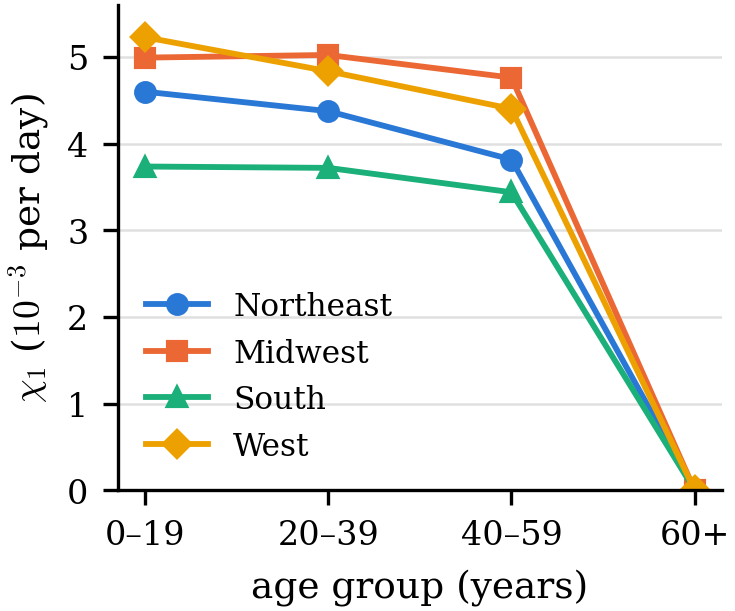
\includegraphics[width=0.4\textwidth]{fig_chi1_min}}\hspace{0.1\textwidth}
\subfloat[John's method, $\rho=2.9312$]{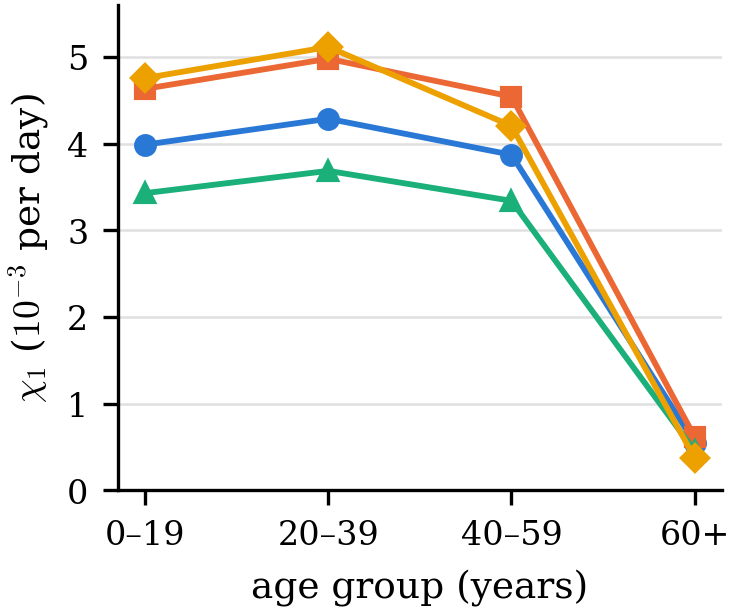
\includegraphics[width=0.4\textwidth]{fig_chi1_john}}
\caption{The minimizer $\chi_1$ and the $\chi_1$ of John's method.}\label{fig-chi1}
\end{figure}

The computations are reproduced by two Mathematica notebooks, which share
their settings. The file \texttt{settings\_zf\_jg.wl} contains the parameters
and the data of~\cite{JZh} and assembles $\operatorname{NGM}$ at $\bm\chi=0$;
both notebooks load it in their first input cell, so that a parameter changed
there changes both. The notebook \texttt{eigenvalues\_H\_ZF\_JG.nb} computes
the spectrum of $\operatorname{NGM}$, $\rho=4.4230681092$ at $\bm\chi=0$, and
John's method: the age profile of the left Perron vector, plotted per location.
The notebook \texttt{min\_rho\_single\_dose\_H\_ZF\_JG.nb} solves the single
dose problem~\eqref{t-program} with the weekly budget $b_{1i}$: an interior
point method in the scaled variables $u_{1,p}$, with the gradient~\eqref{grad},
followed by a quasi-Newton method on the groups that receive doses. It checks
the optimality conditions~\eqref{kkt}, gives the minimum $\rho=2.9059382878$ and
the $\chi_1$ of Table~\ref{tab-chi1}, and compares them with John's method,
$\rho=2.9312317763$, as in Figure~\ref{fig-chi1}. In the single dose numerical tests (see
\texttt{gp\_single\_dose.py}) we solve the same problem by the trust region
interior point method of~\cite{1999Byrd_Hribar_Nocedal}, minimizing
$\log\Psi$, check~\eqref{kkt}, and obtain the same minimum and $\chi_1$.
The fixed point iteration is in \texttt{fixed\_point\_single\_dose.py}.

\section{Optimization for three doses}\label{sec-three}

When doses of the second or third type are available as well, $b_{2i}>0$ or
$b_{3i}>0$ for some $i$, the variables $\bm\chi_2$ and $\bm\chi_3$ do not vanish,
and each $g_p$ in~\eqref{g-def} depends on $\chi_{1,p}$, $\chi_{2,p}$ and
$\chi_{3,p}$. In the variables $\bm u$ of~\eqref{u-of-chihat}
the problem is
\begin{equation}\label{three-program}
\min_{\bm u\in\mathcal{S}}\
\log\rho\left(A_1\operatorname{diag}\left(\bm g\left(\bm\chi(\bm u)\right)\right)\right),
\end{equation}
with $\bm\chi(\bm u)$ given by~\eqref{u-of-chihat} and the
coordinates with $b_{k,i}=0$ equal to zero. The feasible set $\mathcal{S}$ is
the product of the simplices $\Delta_{n-1}$, one for each pair $(k,i)$ with
$b_{k,i}>0$, and the minimum is attained.

The argument of Section~\ref{sec-single} is not available here. The function
$\Phi$ is convex in $\bm\xi=\log\bm g$ by Lemma~\ref{log-convex} in~\S\ref{sec-facts}, but the
objective function of~\eqref{three-program} is $\Phi$ composed with
$\bm u\mapsto\log\bm g\left(\bm\chi(\bm u)\right)$.
For a single dose the proof of Theorem~\ref{global} uses the convexity of each
component of this map; for three doses we have not established it, nor the
convexity of the set $\left\{\log\bm g(\bm\chi):\bm\chi\in\mathfrak{S}\right\}$. Theorem~\ref{global} therefore does not apply
to~\eqref{three-program}, and a local method finds a local minimizer.

In fact the objective function is not convex. The dose $\chi_{2,p}$ enters both
$\pi_{1,p}$, through $\omega_v+\varepsilon_2\chi_{2,p}$, and $\pi_{2,p}$
in~\eqref{yz-def}. For $200\,000$ points $(\chi_{1,p},\chi_{2,p},\chi_{3,p})$
drawn log-uniformly from $\left[10^{-5},10^{-1.5}\right]^3$, with the
parameters of the model, $\varepsilon_1=\varepsilon_2=\varepsilon_3=0.8$ and
$\omega=\omega_v=1/182.5$, the smallest value of
$\chi_{2,p}^2\,\partial^2\log g_p/\partial \chi_{2,p}^2$ is $-0.154$, and $g_p$
increases with $\chi_{2,p}$ at $24.0$ per cent of the points. The equality
constraints therefore cannot be relaxed to inequalities as in
Section~\ref{sec-single}.

In the rest of this section we assume $b_{k,i}>0$ for all $k=1:3$ and
$i=1:m$, and that $A_1\ge 0$ is irreducible.

\subsection{An alternating method}\label{sec-alternating}

Each sweep updates $\bm\chi_1$, $\bm\chi_3$ and $\bm\chi_2$ in turn, the
other two doses fixed at their current values; every iterate satisfies the
constraints~\eqref{constraints}.

\emph{The first dose.} With $\bm\chi_2=\bm\theta$ and $\bm\chi_3=\bm\zeta$
fixed, the minimization of $\Psi(\bm\chi_1,\bm\theta,\bm\zeta)$ over $\bm\chi_1$
is the problem of Section~\ref{sec-single}. Its minimizer is unique
(Theorem~\ref{global}) and is computed by Algorithm~\ref{alg-fixed-point}.

\emph{The third dose.} Let $\bm\chi_1$ and $\bm\chi_2$ be fixed with
$\chi_{1,p}\chi_{2,p}>0$ for all $p$, and let $g^0_p>0$ be the value of
$g_p$ at $\chi_{3,p}=0$. Multiplying the numerator and the denominator
of~\eqref{g-def} by $\omega_v+\varepsilon_2\chi_{2,p}$ and using~\eqref{yz-def},
the numerator does not depend on $\chi_{3,p}$ and the denominator is
$Q^0_p+Q^1_p\chi_{3,p}$ with
\begin{equation*}
Q^0_p=\omega_v+\chi_{1,p}+\varepsilon_2\chi_{2,p}+\frac{2\varepsilon_2}{\omega}\chi_{1,p}\chi_{2,p},\qquad
Q^1_p=\frac{\varepsilon_2\varepsilon_3}{\omega^2}\chi_{1,p}\chi_{2,p}.
\end{equation*}
With $t_p=1+Q^1_p\chi_{3,p}/Q^0_p$ one has $g_p=g^0_p/t_p$, so
\begin{equation}\label{alt-third}
A_1\operatorname{diag}(\bm g)=\left(A_1\operatorname{diag}\left(\bm g^0\right)\right)\operatorname{diag}(\bm t)^{-1}.
\end{equation}
This is~\eqref{t-def} with $e_p=1$ and $A_1$ replaced by the irreducible
matrix $A_1\operatorname{diag}\left(\bm g^0\right)$, and the constraints
of~\eqref{constraints} for $k=3$ become~\eqref{t-constraint} with
$\widetilde\sigma_p=\sigma_{3,p}Q^0_p/\left(\omega_vQ^1_p\right)$ and
$c_i=b_{3i}/\omega_v+\sum_{p\in I_i}\widetilde\sigma_p$. Hence the results of
Section~\ref{sec-single} and Algorithm~\ref{alg-fixed-point} apply to the
minimization over $\bm\chi_3$. If $\chi_{1,p}\chi_{2,p}=0$, then $Q^1_p=0$
and $g_p$ does not depend on $\chi_{3,p}$.

\emph{The second dose.} With $\bm\chi_1=\bm\theta$ and $\bm\chi_3=\bm\zeta$
fixed, the same multiplication gives
$g_p=\left(P^0_p+P^1_p\chi_{2,p}\right)/\left(Q^0_p+Q^1_p\chi_{2,p}\right)$
with $P^0_p=\omega_v+(1-\varepsilon_1)\theta_p$,
$Q^0_p=\omega_v+\theta_p$, $P^1_p=\varepsilon_2\left(1+\theta_p/\omega\right)$
and
$Q^1_p=\varepsilon_2\left(1+2\theta_p/\omega+\varepsilon_3\theta_p\zeta_p/\omega^2\right)$,
so that
$\partial g_p/\partial\chi_{2,p}=-D_p/\left(Q^0_p+Q^1_p\chi_{2,p}\right)^2$ with
\begin{equation}\label{alt-D}
D_p=P^0_pQ^1_p-P^1_pQ^0_p
=\varepsilon_2\theta_p\left(\frac{\omega_v}{\omega}+\omega_vs_p-\varepsilon_1
+\theta_p\left(\frac{1-2\varepsilon_1}{\omega}+(1-\varepsilon_1)s_p\right)\right),\qquad
s_p=\frac{\varepsilon_3\zeta_p}{\omega^2}.
\end{equation}
If $D_p<0$, then $g_p$ increases with $\chi_{2,p}$, and
Section~\ref{sec-single} does not apply. With the parameters of the model,
$\varepsilon_1=\varepsilon_2=\varepsilon_3=0.8$ and $\omega=\omega_v=1/182.5$,
and with $\zeta_p=0$, this is the case whenever $\theta_p>\omega/3$. We minimize
$\Psi(\bm\theta,\bm\chi_2,\bm\zeta)$ over $\bm\chi_2$ by projected Yogi,
\S\ref{sec-yogi}.

The steps for $\bm\chi_1$ and $\bm\chi_3$ return the minimum over their
block, so they do not increase $\rho$; the step for $\bm\chi_2$ is a local
method.

\subsection{Projected Yogi for the second dose}\label{sec-yogi}

In the variables $\bm u$ of~\eqref{u-of-chihat} for $k=2$, the feasible set
of $\bm\chi_2$ is $\mathcal{S}_2=\left(\Delta_{n-1}\right)^m$, and we write
\begin{equation}\label{t-F}
\Theta(\bm u)=\log\Psi\left(\bm\theta,\bm\chi_2(\bm u),\bm\zeta\right),\qquad \bm u\in\mathcal{S}_2 .
\end{equation}
With the eigenvectors $\bm v,\bm w>0$ of~\eqref{perron}, the argument that
gives~\eqref{grad} gives
\begin{equation}\label{t-grad}
\frac{\partial\Theta}{\partial u_{2,ij}}
=\frac{1}{\rho}\cdot\frac{\left(A_1^T\bm w\right)_pv_p}{\langle\bm w,\bm v\rangle}
\cdot\frac{\partial g_p}{\partial \chi_{2,p}}\cdot\frac{b_{2,i}}{\sigma_{2,ij}},
\qquad p=(i-1)n+j .
\end{equation}
For a diagonal $D>0$ of order $N$ let
$\Pi^D_{\mathcal{S}_2}(\bm z)=\operatorname*{arg\,min}_{\bm y\in\mathcal{S}_2}\frac12(\bm y-\bm z)^TD(\bm y-\bm z)$,
and $\Pi_{\mathcal{S}_2}=\Pi^I_{\mathcal{S}_2}$. The problem decouples over the
factors of $\mathcal{S}_2$; in a factor with entries $d_j$ of $D$ the solution
is $y_j=\max\left(z_j-\lambda/d_j,0\right)$, with $\lambda$ the root of
$\sum_j\max\left(z_j-\lambda/d_j,0\right)=1$, which is computed exactly since
the left-hand side is piecewise affine and non-increasing in $\lambda$. As the
measure of stationarity we use
\begin{equation}\label{t-r}
r(\bm u)=\left\|\bm u-\Pi_{\mathcal{S}_2}\left(\bm u-\nabla\Theta(\bm u)\right)\right\|_\infty .
\end{equation}
By the characterization of the projection onto a convex set,
$r(\bm u)=0$ if and only if
$\nabla\Theta(\bm u)^T(\bm x-\bm u)\ge 0$ for all $\bm x\in\mathcal{S}_2$, that
is, $\bm u$ satisfies the Karush--Kuhn--Tucker conditions of the minimization
of $\Theta$ on $\mathcal{S}_2$~\cite[Section 4.2.3]{2004Boyd_Vandenberghe}.

Algorithm~\ref{t-alg-yogi} states the method. Squares, square roots, products,
quotients and $\operatorname{sign}$ of vectors are taken entrywise. Compared
with the method as stated in~\cite{2018Zaheer_Yogi}, the gradient is exact
rather than stochastic, and the step is followed by the projection; we start
the second moment $\bm s$ at the square of the first gradient, and divide the
first moment $\bm\kappa$ by $1-\beta_1^t$.

\begin{algorithm}[ht]
\caption{Projected Yogi}\label{t-alg-yogi}
\begin{algorithmic}[1]
\Require a start $\bm u^{(0)}\in\mathcal{S}_2$; a step $\eta>0$;
$\beta_1\in[0,1)$, $\beta_2\in(0,1)$, $\epsilon>0$; a tolerance $\mathrm{tol}$
and a maximal number of iterations $t_{\max}$
\State $\bm q\gets\nabla\Theta\left(\bm u^{(0)}\right)$, $\bm\kappa\gets\bm 0$, $\bm s\gets\bm q^2$
\For{$t=1,\ldots,t_{\max}$}
  \State $\bm q\gets\nabla\Theta\left(\bm u^{(t-1)}\right)$
  \State $\bm\kappa\gets\beta_1\bm\kappa+(1-\beta_1)\bm q$
  \State $\bm s\gets\bm s-(1-\beta_2)\operatorname{sign}\left(\bm s-\bm q^2\right)\bm q^2$
  \State $D\gets\operatorname{diag}\left(\sqrt{\bm s}+\epsilon\right)$
  \State $\bm u^{(t)}\gets\Pi^D_{\mathcal{S}_2}\left(\bm u^{(t-1)}-\eta D^{-1}\bm\kappa/\left(1-\beta_1^t\right)\right)$
  \If{$r\left(\bm u^{(t)}\right)<\mathrm{tol}$}
    \State \textbf{break}
  \EndIf
\EndFor
\State \Return $\bm u^{(t)}$, $\rho=\exp\Theta\left(\bm u^{(t)}\right)$
\end{algorithmic}
\end{algorithm}

We do not prove that the iterates converge.

\subsection{Numerical results}\label{sec-three-numerics}

{\color{red} ZF: Thanks, Ludmil. The Theorems and proofs look very fancy, but it may take time for me to understand all the notation and changes of variables. I am now just commenting on the numerical results and assumptions on vaccine doses.
The results about a single dose ($\chi_1$) look great. For the second dose ($\chi_2$), I am not sure how you did it. For the applications in our model, notice that the numbers of vaccine doses in the constraints are weekly numbers, and the numbers of susceptibles (S) and vaccined with dose 1 (V) will change at the end of the week after applied the optimal allocations. So, we will need to calculate the new S and V first, and then based on the updated S and V to determine the optimal $\chi_1$ and $\chi_2$ for the following week.
}

The computations start with the trust region interior point method
of~\cite{1999Byrd_Hribar_Nocedal} in all $3N$ variables $\bm u$, with the
gradient computed as in~\eqref{t-grad} for each $k$, for at most $500$
iterations. If the method stops earlier by its own tolerances, its point is
the result. Otherwise the alternating method of~\S\ref{sec-alternating} is
started from its point and stopped when $r<10^{-10}$, where $r$ is defined
as in~\eqref{t-r} with all $3N$ variables in place of those of
$\bm\chi_2$; by the product structure of the constraints, a point at which
no step of the alternating method changes the iterate satisfies the
Karush--Kuhn--Tucker conditions in all $3N$ variables. In the steps for
$\bm\chi_1$ and $\bm\chi_3$, Algorithm~\ref{alg-fixed-point} stops at the
relative change $10^{-13}$; in the step for $\bm\chi_2$,
Algorithm~\ref{t-alg-yogi} has $\eta=10^{-2}$, $\beta_1=0.9$,
$\beta_2=0.999$, $\epsilon=10^{-8}$, $\mathrm{tol}=10^{-11}$ and
$t_{\max}=2\cdot 10^4$.

\paragraph{Instances and starts.} In the weekly instance the budget $b_{1i}$
and $\sigma_{1,ij}$ are those of Section~\ref{sec-numerics}; no budget for the
second and third doses is given with the data of~\cite{JZh}, and we take
$b_{2i}=b_{3i}=b_{1i}/4$ and $\sigma_{2,ij}=\sigma_{3,ij}=P_{ij}$, the numbers
of partially protected individuals. The $36$ instances vary these data: the
budget $b_{1i}$ weekly or daily ($b_{1i}/7$); the ratios
\begin{equation*}
\frac{(b_{2i},b_{3i})}{b_{1i}}\in\left\{\left(\tfrac1{16},\tfrac1{16}\right),\left(\tfrac14,\tfrac14\right),(1,1),(4,4),\left(\tfrac12,\tfrac18\right),\left(\tfrac18,\tfrac12\right)\right\};
\end{equation*}
and $\sigma_{2,ij}$, $\sigma_{3,ij}$ equal to $P_{ij}$, or to
$P_{ij}e^{Z_{ij}/2}$ and $P_{ij}e^{Z'_{ij}/2}$ with independent standard normal
$Z$, $Z'$, for two seeds. Seed $s\in\{1,2\}$ means that $Z$ and then $Z'$, each
$m\times n$ with the entries in row order, are drawn by
\texttt{numpy.random.default\_rng(s).standard\_normal}. Each instance is run
from $49$ starts: the barycenter $\overline{\bm u}$ of $\mathcal{S}$,
$\overline u_{k,ij}=1/n$, and the $3mn=48$ points obtained from it by
replacing one factor $(k,i)$ with $(1-\delta)\bm e_j+\delta\mathbbm{1}/n$,
$\delta=10^{-3}$; in the start $(k,i,j)$ all doses of type $k$ in location $i$
go, up to $\delta$, to the age group $j$. For each instance $\rho_{\mathrm{ref}}$
is the smallest value of $69$ runs of the trust region method to its own
tolerances, from these $49$ starts and from $20$ random points of
$\mathcal{S}$, and a run ends at $\rho_{\mathrm{ref}}$ if its value is at most
$\left(1+10^{-7}\right)\rho_{\mathrm{ref}}$. In two weekly instances,
$b_{2i}=b_{3i}=b_{1i}/4$ with $\sigma_2$, $\sigma_3$ of seed $2$, and
$b_{2i}=b_{1i}/8$, $b_{3i}=b_{1i}/2$ with $\sigma_2=\sigma_3=P$,
Algorithm~\ref{t-alg-yogi} applied in all $3N$ variables from the barycenter
ends below $\rho_{\mathrm{ref}}$, by $0.13$ and $0.025$ per cent, so
$\rho_{\mathrm{ref}}$ is not the minimum in every instance.

\paragraph{The weekly instance.} From all $49$ starts the method ends at
$\rho=1.6618260420$, within $4.3\cdot 10^{-9}$ relative of
$\rho_{\mathrm{ref}}$. Table~\ref{t-tab-tralt} gives the trust region
iterations and the times. The trust region method stops by its own tolerances
in $48$ runs; in the run from the start $(2,4,1)$ it reaches $500$ iterations
and the alternating method ends after $8$ sweeps.

\begin{table}[ht]
\centering
\small
\begin{tabular}{lcccc}
\hline
starts & barycenter & dose $1$ at a vertex & dose $2$ at a vertex & dose $3$ at a vertex\\
 & ($1$) & ($16$) & ($16$) & ($16$)\\
\hline
trust region iterations & $130$ & $173$--$321$ & $174$--$500$ & $126$--$238$\\
alternating method used & $0$ & $0$ & $1$ & $0$\\
time & $0.5$ s & $14.1$ s & $18.8$ s & $10.8$ s\\
\hline
\end{tabular}
\caption{The weekly instance from the $49$ starts; the times are totals over
the starts of each column, with $12$ runs in parallel.}\label{t-tab-tralt}
\end{table}

\paragraph{Thirty-six instances.} In every instance the smallest value of the
$49$ runs is $\rho_{\mathrm{ref}}$; all $49$ runs take $40$ s per instance on
average, and all $36\cdot 49=1764$ runs take $163$ s with $12$ runs in
parallel, $1430$ s in total, median $0.56$ s per run. The run from the
barycenter alone ends at $\rho_{\mathrm{ref}}$ in $33$ instances.

Of the $1764$ runs, $1572$ end at $\rho_{\mathrm{ref}}$. The trust region
method reaches $500$ iterations in $110$ runs; in all of them the alternating
method ends at $\rho_{\mathrm{ref}}$, after between $3$ and $29$ sweeps,
median $6$. The $192$ runs that do not end at $\rho_{\mathrm{ref}}$ are runs in
which the trust region method stops by its own tolerances, so that the
alternating method is not used, between $68$ and $266$ iterations, above $\rho_{\mathrm{ref}}$
by between $6.7\cdot 10^{-5}$ and $1.3\cdot 10^{-2}$ relative, with $r$ at most
$1.8\cdot 10^{-7}$ and median $1.7\cdot 10^{-10}$. These are points satisfying
the Karush--Kuhn--Tucker conditions to this accuracy with different values of
the objective function; for a convex differentiable function on a convex set
every such point is a global minimizer~\cite[Section 4.2.3]{2004Boyd_Vandenberghe},
so the objective function is not convex on these instances, and the
alternating method, started at such a point, does not change it. In $24$
instances all $49$ runs end at $\rho_{\mathrm{ref}}$;
Table~\ref{t-tab-tralt-miss} lists the other $12$.

\begin{table}[ht]
\centering
\small
\begin{tabular}{llccc}
\hline
budget & $(b_{2i},b_{3i})/b_{1i}$ & $\sigma_2,\sigma_3$ & runs at $\rho_{\mathrm{ref}}$ & largest relative excess\\
\hline
daily  & $(\tfrac18,\tfrac12)$       & $P$      & $1^*$  & $3.2\cdot 10^{-3}$\\
weekly & $(\tfrac1{16},\tfrac1{16})$ & seed $2$ & $1^*$  & $5.4\cdot 10^{-3}$\\
daily  & $(\tfrac1{16},\tfrac1{16})$ & $P$      & $10^*$ & $1.1\cdot 10^{-4}$\\
daily  & $(\tfrac14,\tfrac14)$       & $P$      & $16$   & $2.0\cdot 10^{-3}$\\
daily  & $(\tfrac14,\tfrac14)$       & seed $2$ & $38$   & $5.1\cdot 10^{-4}$\\
daily  & $(\tfrac18,\tfrac12)$       & seed $2$ & $46$   & $1.3\cdot 10^{-2}$\\
daily  & $(\tfrac12,\tfrac18)$       & seed $1$ & $46$   & $2.2\cdot 10^{-3}$\\
weekly & $(\tfrac1{16},\tfrac1{16})$ & $P$      & $46$   & $1.2\cdot 10^{-2}$\\
daily  & $(\tfrac1{16},\tfrac1{16})$ & seed $2$ & $48$   & $7.4\cdot 10^{-4}$\\
daily  & $(\tfrac18,\tfrac12)$       & seed $1$ & $48$   & $8.4\cdot 10^{-3}$\\
daily  & $(\tfrac14,\tfrac14)$       & seed $1$ & $48$   & $5.0\cdot 10^{-3}$\\
daily  & $(1,1)$                     & seed $1$ & $48$   & $4.8\cdot 10^{-3}$\\
\hline
\end{tabular}
\caption{The instances in which not all $49$ runs end at $\rho_{\mathrm{ref}}$:
the number of runs that do, out of $49$, with $^*$ where the run from the
barycenter does not, and the largest relative excess
$(\rho-\rho_{\mathrm{ref}})/\rho_{\mathrm{ref}}$ over the $49$
runs.}\label{t-tab-tralt-miss}
\end{table}

Figure~\ref{t-fig-tralt-conv} shows, for the weekly instance with
$b_{2i}=b_{1i}/8$, $b_{3i}=b_{1i}/2$ and $\sigma_2=\sigma_3=P$, in which the
trust region method reaches $500$ iterations from $41$ of the $49$ starts, the
relative excess $(\rho-\rho_{\mathrm{ref}})/\rho_{\mathrm{ref}}$ per trust
region iteration from the barycenter and from the starts $(1,1,4)$ and
$(2,4,4)$, and the relative excess and $r$ per sweep of the alternating method
started after $500$ iterations from the latter two. From the barycenter the
trust region method stops after $121$ iterations. From $(1,1,4)$ and $(2,4,4)$,
after $500$ iterations the excess is $1.6\cdot 10^{-8}$ and $2.3\cdot 10^{-7}$
and $r$ is $6.2\cdot 10^{-6}$ and $1.4\cdot 10^{-5}$. The first sweep of the
alternating method brings $\rho$ below $\rho_{\mathrm{ref}}$, each further
sweep reduces $r$ by a factor between $5$ and $21$, and $r<10^{-10}$ after $6$
and $7$ sweeps. Excesses below
$10^{-16}$, including the negative excesses of the endpoints, which lie
$1.1\cdot 10^{-10}$ relative below $\rho_{\mathrm{ref}}$, are shown at
$10^{-16}$.

\begin{figure}[!ht]
\centering
\subfloat[trust region iterations]{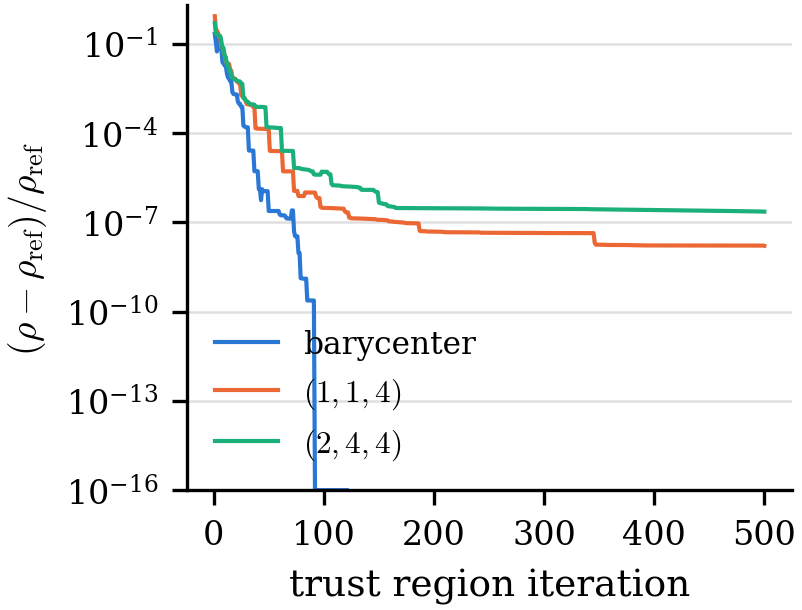
\includegraphics[width=0.34\textwidth]{fig_tralt_tr}}\hspace{0.1\textwidth}
\subfloat[sweeps of the alternating method]{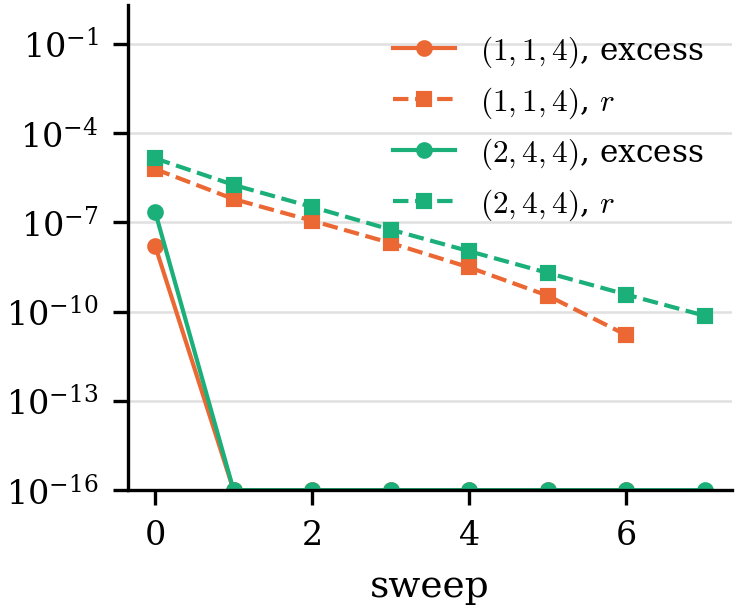
\includegraphics[width=0.34\textwidth]{fig_tralt_alt}}
\caption{The weekly instance with $b_{2i}=b_{1i}/8$, $b_{3i}=b_{1i}/2$ and
$\sigma_2=\sigma_3=P$ from three starts.}\label{t-fig-tralt-conv}
\end{figure}

Figure~\ref{t-fig-alloc-tralt} shows the allocations $\chi_{k,ij}$ at the
endpoint from the barycenter, in units of $10^{-3}$ per day, one line per
location, for the weekly instance, $\rho=1.6618$, and for the weekly instance
with $b_{2i}=b_{1i}/8$, $b_{3i}=b_{1i}/2$ and $\sigma_2=\sigma_3=P$,
$\rho=1.3088$. In the first the group $60+$ receives no doses of any type in
the Northeast, the South and the West, and in the Midwest it receives first
and second doses but no third doses. In the second every group receives first
doses, and the group $60+$ of the Northeast and of the South receives no
second or third doses. As for the single dose, where the group $60+$ receives
no doses at the minimizer, doses go away from this group.

\begin{figure}[!htbp]
\centering
\subfloat[$\chi_1$, weekly instance]{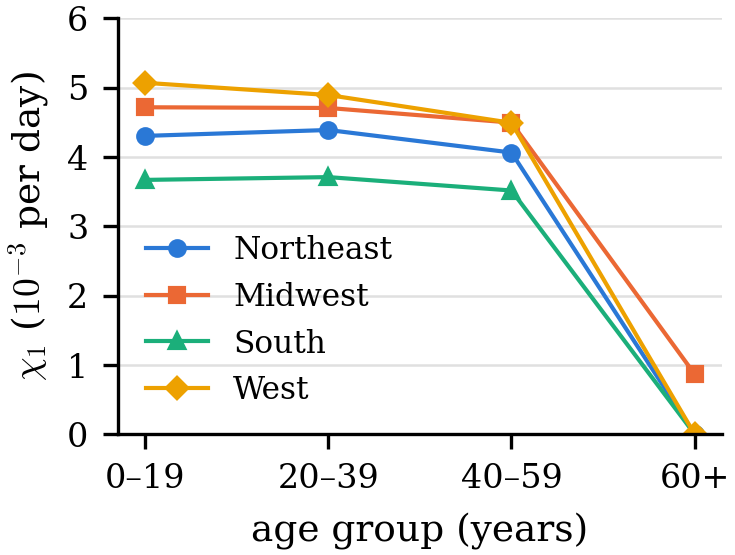
\includegraphics[width=0.28\textwidth]{fig_alloc_tralt_q_k1}}\hfill
\subfloat[$\chi_2$, weekly instance]{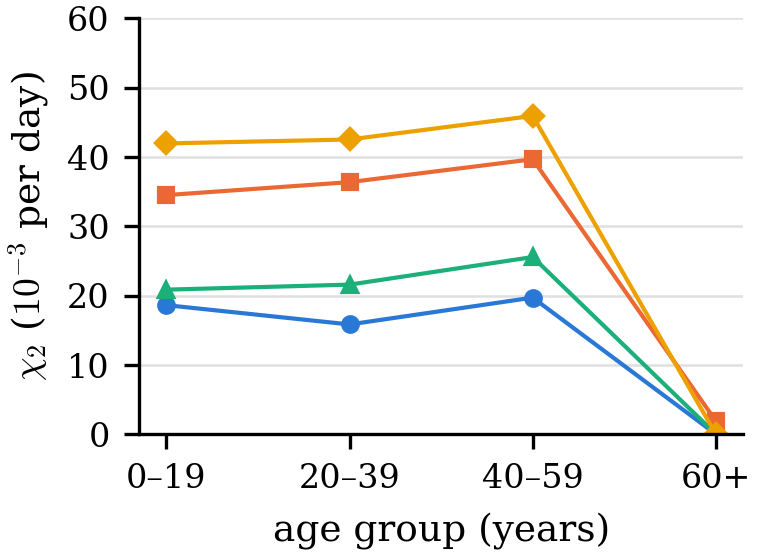
\includegraphics[width=0.28\textwidth]{fig_alloc_tralt_q_k2}}\hfill
\subfloat[$\chi_3$, weekly instance]{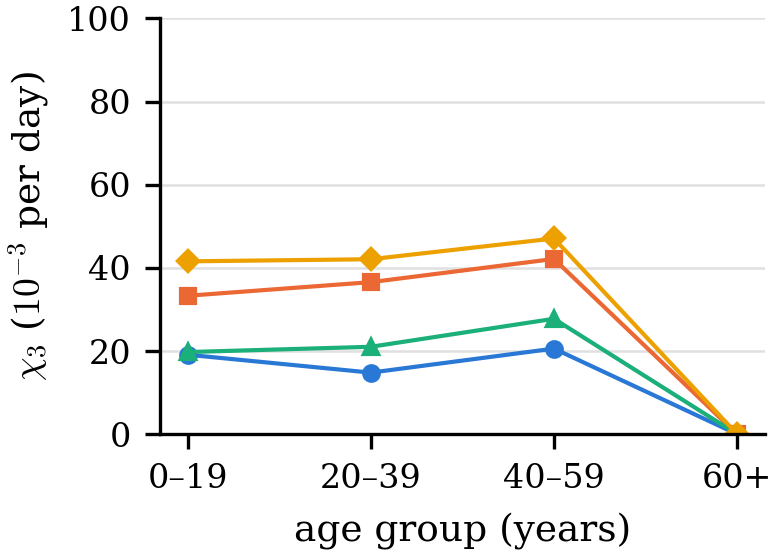
\includegraphics[width=0.28\textwidth]{fig_alloc_tralt_q_k3}}\\
\subfloat[$\chi_1$, second instance]{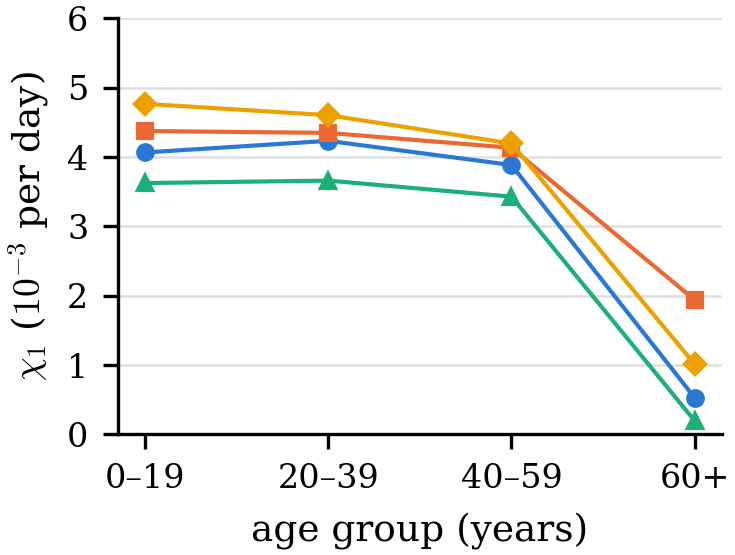
\includegraphics[width=0.28\textwidth]{fig_alloc_tralt_p_k1}}\hfill
\subfloat[$\chi_2$, second instance]{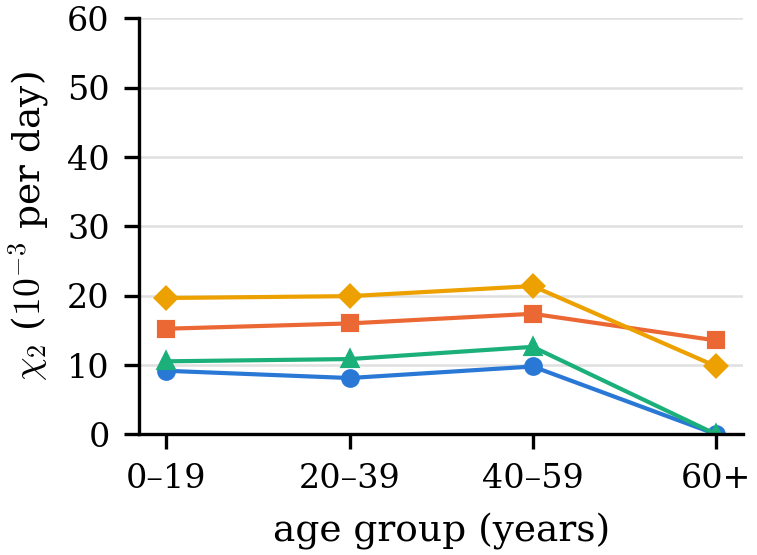
\includegraphics[width=0.28\textwidth]{fig_alloc_tralt_p_k2}}\hfill
\subfloat[$\chi_3$, second instance]{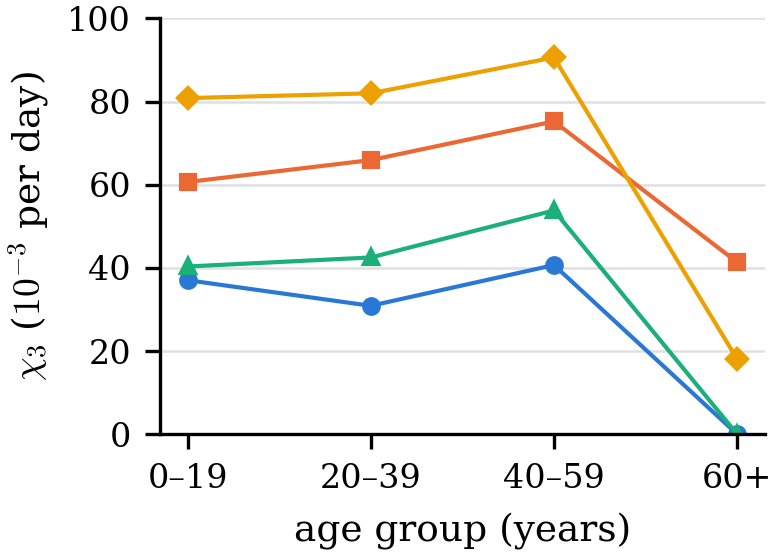
\includegraphics[width=0.28\textwidth]{fig_alloc_tralt_p_k3}}
\caption{The allocations at the endpoint from the barycenter. Top row: the
weekly instance, $b_{2i}=b_{3i}=b_{1i}/4$, $\sigma_2=\sigma_3=P$,
$\rho=1.6618$. Bottom row: $b_{2i}=b_{1i}/8$, $b_{3i}=b_{1i}/2$,
$\sigma_2=\sigma_3=P$, $\rho=1.3088$.}\label{t-fig-alloc-tralt}
\end{figure}

The computations are in the following python files:
\begin{itemize}
\item \texttt{alt\_three\_dose.py}: the alternating method;
\item \texttt{tr\_alt\_instances\_three\_dose.py}: the $36$ instances from the
$49$ starts, and Tables~\ref{t-tab-tralt} and~\ref{t-tab-tralt-miss};
\item \texttt{plot\_tr\_alt\_three\_dose.py}: the data of
Figures~\ref{t-fig-tralt-conv} and~\ref{t-fig-alloc-tralt}.
\end{itemize}

\FloatBarrier
\appendix

\section{On the equivalence of the two formulations}\label{sec-reduction}

Recall $\mathscr{P}$ from~\eqref{p-def} and~\eqref{p-identities}. 
Given with $\bm{a}\in \mathbb{R}^{N}$ we call a diagonal matrix
$X(\bm a)=\operatorname{diag}\left(\bm x(\bm a)\right)
\in\mathbb{R}^{2N\times 2N}$ 
\emph{doubled} if $x_{2p-1}=x_{2p}=a_p$; 
a direct computation gives $X\mathscr{P}=\mathscr{P}\operatorname{diag}(\bm a)$ and
$\mathscr{P}^TX=\operatorname{diag}(\bm a)\mathscr{P}^T$. Further, let $\bm d_c\in\mathbb{R}^{N}$, $N=mn$ is composed from the entries of the product 
\begin{equation}
d_{c,p}=\left\lbrack\operatorname{diag}(\bm s)\,\mathscr{A}\,
\operatorname{diag}\left(\bm\psi_S\odot\bm\beta\right)\right\rbrack_{ij},
\qquad p=(i-1)n+j,
\end{equation} 
$D_0$ be the doubled diagonal matrix with underlying vector $\bm d_c$. 
The definition of $\operatorname{NGM}$ in~\cite{JZh} uses the constant matrix $A_c$ such that 
\begin{equation}\label{ac-assembled}
A_c=D_0\left(\mathscr{P}C\mathscr{P}^T\right)\Psi_IQ.
\end{equation}
Here, $C\in\mathbb{R}^{N\times N}$ is the mixing matrix and $\Psi_I(\bm\psi_I)$, and $Q(\bm q)$ 
are doubled diagonal matrices of order $2N$, with given
$\bm\psi_I,\bm q\in\mathbb{R}^{N}$.
A straightforward computation gives
\begin{equation}\label{a1-explicit}
A_c=\mathscr{P}A_1\mathscr{P}^T\qquad\mbox{with}\qquad
A_1=\operatorname{diag}(\bm d_c)\,C\operatorname{diag}\left(\bm\psi_I\odot\bm q\right),
\end{equation}
where $\odot$ is the entry-wise product. In particular $A_1>0$ whenever $C$,
$\bm d_c$, $\bm\psi_I$ and $\bm q$ are positive, which holds for the data we consider~\cite{JZh}. Indeed,
substituting in~\eqref{ac-assembled} and using the identities for doubled
matrices, $D_0\mathscr{P}=\mathscr{P}\operatorname{diag}(\bm d_c)$ and
$\mathscr{P}^T\Psi_IQ=\operatorname{diag}\left(\bm\psi_I\odot\bm q\right)\mathscr{P}^T$,
gives~\eqref{a1-explicit}. Multiplying the first identity
in~\eqref{a1-explicit} by $\mathscr{P}^T$ on the left and by $\mathscr{P}$ on the
right and using $\mathscr{P}^T\mathscr{P}=2I_N$ twice, we obtain the definition
of $A_1$ in~\eqref{p-identities}.


Next, we consider the quantities $y_p$ and $z_p$ of~\eqref{yz-def}. Adding
them we find the closed form of $g_p$ in~\eqref{g-def}. Moreover, since $\widetilde s_p\in(0,1]$, one has $0<g_p\le 1$, with $g_p=1$ exactly when $\chi_{1,p}=0$.

We also have the following identity: $\bm d$ as in~\eqref{yz} and $\bm g=\bm y+\bm z$,
\begin{equation}\label{ptdp}
\mathscr{P}^T\operatorname{diag}(\bm d)\mathscr{P}=\operatorname{diag}(\bm g).
\end{equation}
To see this, 
we observe that 
$\left(\mathscr{P}^T\operatorname{diag}(\bm d)\mathscr{P}\right)_{pl}
=\sum_{r}\mathscr{P}_{rp}d_r\mathscr{P}_{rl}$. Since $\mathscr{P}_{rp}\neq 0$ only
for $r\in\{2p-1,2p\}$, this sum vanishes for $p\neq l$. For $p=l$, it equals $d_{2p-1}+d_{2p}=y_p+z_p$ which is what we wanted to show.

Next theorem was used in the main text to reduce the order of the matrix in the spectral radius minimization problem.
Recall that $\bm d\in\mathbb{R}^{2N}$ and $\bm g\in\mathbb{R}^{N}$ are related by $\bm g=\mathscr{P}^T\bm d$.
\begin{theorem}\label{reduction}
The following identity holds
\begin{equation}
\rho\left(\operatorname{diag}(\bm d)A_c\right)=\rho\left(A_1\operatorname{diag}(\bm g)\right).
\end{equation}
Moreover, any non-zero eigenvalue of $\operatorname{diag}(\bm d)A_c$ is also an
eigenvalue of $A_1\operatorname{diag}(\bm g)$, and vice versa.
\end{theorem}
\begin{proof}
By~\eqref{a1-explicit} and~\eqref{ptdp},
\begin{equation}\label{two-products}
\operatorname{diag}(\bm d)A_c=\operatorname{diag}(\bm d)\mathscr{P}A_1\mathscr{P}^T,
\qquad
A_1\operatorname{diag}(\bm g)=A_1\mathscr{P}^T\operatorname{diag}(\bm d)\mathscr{P}.
\end{equation}
Let $\lambda\neq 0$. If $A_1\operatorname{diag}(\bm g)\bm v=\lambda\bm v$ with
$\bm v\neq 0$, put $\bm x=\operatorname{diag}(\bm d)\mathscr{P}\bm v$. Then
\begin{equation}
\operatorname{diag}(\bm d)A_c\,\bm x
=\operatorname{diag}(\bm d)\mathscr{P}\left(A_1\mathscr{P}^T\operatorname{diag}(\bm d)\mathscr{P}\bm v\right)
=\lambda\,\bm x,
\end{equation}
and $\bm x\neq 0$, since $A_1\mathscr{P}^T\bm x=\lambda\bm v\neq 0$.
Conversely, if $\operatorname{diag}(\bm d)A_c\bm x=\lambda\bm x$ with
$\bm x\neq 0$, put $\bm v=A_1\mathscr{P}^T\bm x$. Then
\begin{equation}
A_1\operatorname{diag}(\bm g)\,\bm v
=A_1\mathscr{P}^T\left(\operatorname{diag}(\bm d)\mathscr{P}A_1\mathscr{P}^T\bm x\right)
=\lambda\,\bm v,
\end{equation}
and $\bm v\neq 0$, since $\operatorname{diag}(\bm d)\mathscr{P}\bm v=\lambda\bm x\neq 0$.
So the two matrices have the same non-zero eigenvalues. This implies that two spectral radii are equal.
\end{proof}

\section{Some well known facts about non-negative matrices}\label{sec-facts}

\begin{theorem}[Perron--Frobenius]\label{pf}
Let $A\ge 0$ be irreducible. Then $\rho(A)>0$ is a simple eigenvalue of $A$,
and the corresponding eigenvector has positive components.
\end{theorem}

For a proof see Varga~\cite[Theorem 2.7]{2000Varga-aa}; for the next
theorem see~\cite[Section 8.1]{1985Horn_Johnson}.

\begin{theorem}\label{mono}
Let $0\le B\le A$. Then $\rho(B)\le\rho(A)$, and $\rho(B)<\rho(A)$ if in
addition $A$ is irreducible and $B\neq A$.
\end{theorem}

\begin{lemma}\label{log-convex}
Let $A\ge 0$ with $\rho(A)>0$ and set
\begin{equation}\label{phi-def}
\Phi(\bm\xi)=\log\rho\left(A\operatorname{diag}\left(e^{\bm\xi}\right)\right).
\end{equation}
Then $\Phi$ is convex.
\end{lemma}
\begin{proof}
$\Phi$ is finite: with $c=\min_l e^{\xi_l}>0$ we have
$cA\le A\operatorname{diag}\left(e^{\bm\xi}\right)$, so by Theorem~\ref{mono}
\begin{equation}
\rho\left(A\operatorname{diag}\left(e^{\bm\xi}\right)\right)\ge c\,\rho(A)>0.
\end{equation}
We first prove the lemma for irreducible $A$ in Steps 1--3, and then remove
this assumption in Step 4.

An irreducible matrix has no zero row (with the index of a zero row placed
last, the matrix would be block upper triangular), so for every $p$ the set
$\mathcal{L}_p=\{l:A_{pl}>0\}$ is not empty. For $\bm\xi,\bm\zeta\in\mathbb{R}^N$
let
\begin{equation}\label{cw-F}
\begin{aligned}
F(\bm\xi,\bm\zeta)&=\max_{p}\,h_p(\bm\xi,\bm\zeta),\qquad\mbox{where}\\
h_p(\bm\xi,\bm\zeta)&=\log\frac{\left(A\operatorname{diag}\left(e^{\bm\xi}\right)e^{\bm\zeta}\right)_p}{e^{\zeta_p}}\\
&=\log\sum_{l\in\mathcal{L}_p}\exp\left(\log A_{pl}+\xi_l+\zeta_l-\zeta_p\right).
\end{aligned}
\end{equation}

\emph{Step 1: $\Phi(\bm\xi)=\min_{\bm\zeta}F(\bm\xi,\bm\zeta)$.} Fix $\bm\xi$
and put $A_e=A\operatorname{diag}\left(e^{\bm\xi}\right)$. Since $e^{\bm\xi}>0$,
the matrix $A_e\ge 0$ has the same zero entries as $A$, so $A_e$ and $A_e^T$ are
irreducible, and by Theorem~\ref{pf} there are $\bm v>0$ and $\bm w>0$ with
$A_e\bm v=\rho(A_e)\bm v$ and $A_e^T\bm w=\rho(A_e)\bm w$. For $\bm\zeta=\log\bm v$
every $h_p$ equals $\log\rho(A_e)$, so $F(\bm\xi,\log\bm v)=\Phi(\bm\xi)$. For
any $\bm\zeta$, put $\bm x=e^{\bm\zeta}>0$ and $\theta=e^{F(\bm\xi,\bm\zeta)}$;
then $A_e\bm x\le\theta\bm x$, and pairing with $\bm w>0$,
\begin{equation}
\rho(A_e)\langle\bm w,\bm x\rangle=\langle A_e^T\bm w,\bm x\rangle
=\langle\bm w,A_e\bm x\rangle\le\theta\langle\bm w,\bm x\rangle .
\end{equation}
As $\langle\bm w,\bm x\rangle>0$, $\rho(A_e)\le\theta$, that is,
$\Phi(\bm\xi)\le F(\bm\xi,\bm\zeta)$.

\emph{Step 2: $F$ is jointly convex in $(\bm\xi,\bm\zeta)$.} Each $e^{h_p}$ is
a sum of functions $\exp\left(a_l(\bm\xi,\bm\zeta)\right)$ with $a_l$ affine.
For $0\le\lambda\le 1$ and two points, write $f_l$ and $g_l$ for the values of
$\exp(a_l)$ at the two points; since $a_l$ is affine, the value at the convex
combination is $f_l^{\lambda}g_l^{1-\lambda}$, and by H\"older's inequality
with exponents $1/\lambda$ and $1/(1-\lambda)$,
\begin{equation}
\sum_l f_l^{\lambda}g_l^{1-\lambda}\le\Big(\sum_l f_l\Big)^{\lambda}\Big(\sum_l g_l\Big)^{1-\lambda}.
\end{equation}
Taking logarithms, the value of $h_p$ at the convex combination is at most
$\lambda$ times its value at the first point plus $1-\lambda$ times its value
at the second, so $h_p$ is convex, and $F$, a maximum of convex functions, is
convex.

\emph{Step 3.} Let $\bm\xi,\bm\eta\in\mathbb{R}^N$, $0\le\lambda\le 1$, and by
Step 1 choose $\bm\zeta$ and $\bm\zeta'$ with $F(\bm\xi,\bm\zeta)=\Phi(\bm\xi)$
and $F(\bm\eta,\bm\zeta')=\Phi(\bm\eta)$. By Steps 1 and 2,
\begin{equation}
\Phi\left(\lambda\bm\xi+(1-\lambda)\bm\eta\right)
\le F\left(\lambda\bm\xi+(1-\lambda)\bm\eta,\ \lambda\bm\zeta+(1-\lambda)\bm\zeta'\right)
\le\lambda\Phi(\bm\xi)+(1-\lambda)\Phi(\bm\eta).
\end{equation}

\emph{Step 4: $A\ge 0$ not irreducible.} For $\varepsilon>0$ the matrix
$A_\varepsilon=A+\varepsilon\mathbbm{1}\mathbbm{1}^T$ is positive, hence
irreducible, so by Steps 1--3 the function
$\Phi_\varepsilon(\bm\xi)=\log\rho\left(A_\varepsilon\operatorname{diag}\left(e^{\bm\xi}\right)\right)$
is convex. The spectral radius depends continuously on the entries of the
matrix, and $\rho\left(A\operatorname{diag}\left(e^{\bm\xi}\right)\right)>0$, so
$\Phi_\varepsilon(\bm\xi)\to\Phi(\bm\xi)$ as $\varepsilon\to 0$ for every
$\bm\xi$. A pointwise limit of convex functions is convex.
\end{proof}

\bibliographystyle{plain}
\bibliography{bib_mb}

\end{document}
